%% Ankur Sinha

%% packages %%
% support for coloured text
\usepackage{color}
% IPA
\usepackage{tipa}
\usepackage[scale=2]{ccicons}
\usepackage{amssymb}
\usepackage{tikz}
\usetikzlibrary{arrows.meta, arrows}
\usepackage{pgfplots}
\pgfmathdeclarefunction{gaussnew}{4}{%nu, eta, eps, omega
  \pgfmathparse{(#1*((2*exp(-(((x-((#2+#3)/2))/((#2-#3)/(2*sqrt(-ln(#4/2)))))^2))) -#4))}%chktex 36
}
\usepackage{jneurosci}
\usepackage{subfig}
\usepackage[T1]{fontenc}
\usepackage[utf8]{inputenc}
\usepackage[style=nature,backend=biber,autocite=footnote]{biblatex}
\addbibresource{/home/asinha/Documents/01_Readables/00_research_papers/masterbib.bib}
% Use opensans
\usepackage[default,osfigures,scale=0.95]{opensans}
% for strike through
\usepackage[normalem]{ulem}
% links, urls, refs
\definecolor{links}{HTML}{2A1B81}
% Fedora blue for the theme
\definecolor{FedoraBlue}{HTML}{2A1B81}
\usepackage{hyperref}
\hypersetup{colorlinks,linkcolor=Green,urlcolor=links}
% graphics
\usepackage{graphicx}
% algorithm
\usepackage{algorithmic}
\usepackage{textcomp}
\usepackage{wrapfig}
\usepackage{textgreek}
\usepackage{euler}

% beamer theme
% use defaults for theme
\usetheme[numbering=fraction]{metropolis}
\usefonttheme[onlymath]{serif}
\setbeamerfont{footnote}{size=\tiny}
\setbeamerfont{caption}{size=\tiny}
\setbeamercolor{alerted text}{fg=Green}
\setbeamerfont{note page}{size=\small}

% Not needed in metropolis, but in general footnote citation fixes: https://tex.stackexchange.com/questions/44217/how-can-i-stop-footcite-from-hijacking-my-beamer-columns
% how to use multiple references to the same footnote: https://tex.stackexchange.com/questions/27763/beamer-multiple-references-to-the-same-footnote

%% title %%
\title{Investigating the activity dependent dynamics of synaptic structures using biologically realistic modelling of peripheral lesion experiments}
\subtitle{Discussion of my Ph.D. research}
\author[Ankur Sinha]{Ankur Sinha}
\date{29/03/2019}

%% document begins %%
\begin{document}

% title frame %%
\begin{frame}
  \titlepage{}
\end{frame}

%% Three slides for 5 minutes seems good
%% So, 30 slides at most for 50 minutes
\section{Context}
\begin{frame}[c]{Plasticity while maintaining stability}
  \begin{figure}[h]
    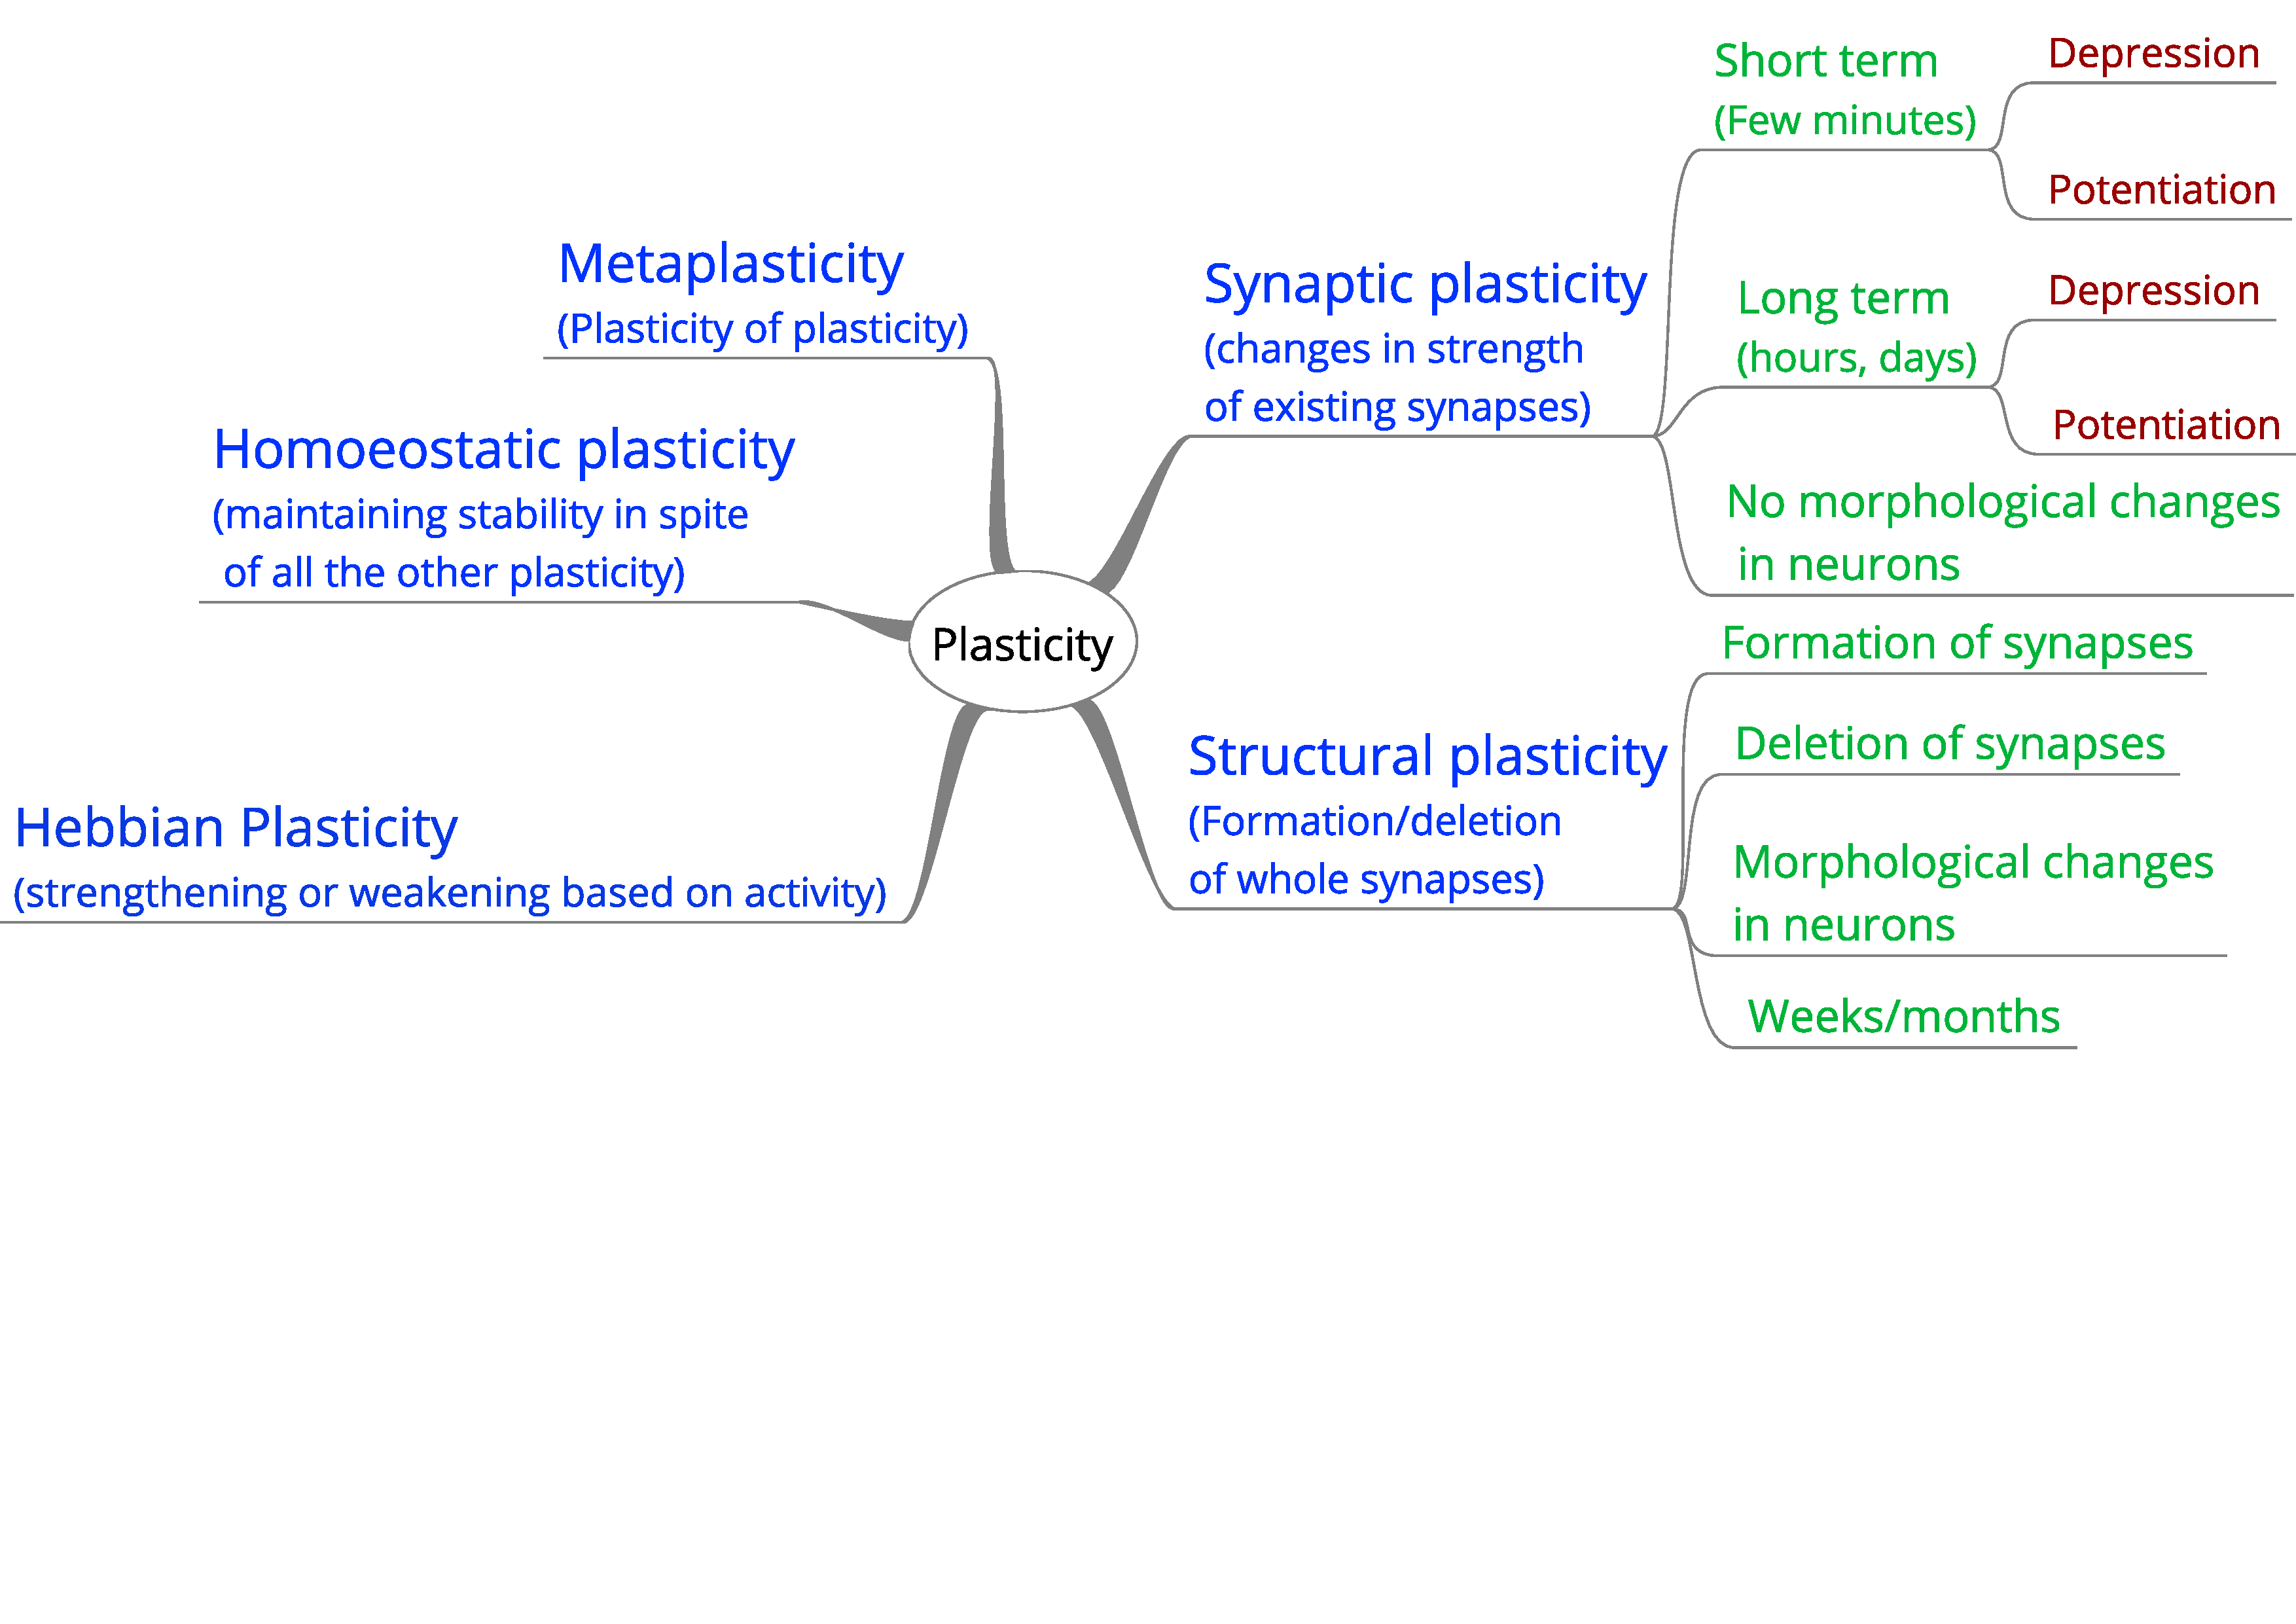
\includegraphics[width=1.05\linewidth]{99_images/Plasticity.pdf}
  \end{figure}
  \note[item]{We know there are multiple plasticity mechanisms active all at once. Hebbian plasticity underlies learning, but de-stabilises networks. Homeostatic plasticity ensures that even when learning occurs, the network remains in a stable state}
  \note[item]{Generally, though, when we speak of these, we refer to synaptic plasticity only. But, lots of evidence now confirms that, in fact, structural plasticity is active in the adult brain. So not only are synaptic weights changing, the connectivity of networks is changing too!}
  \note[item]{So, it isn't hard to imaging how if changes in synaptic strengths makes plasticity-stability an issue, how the removal and formation of whole synapses would have a much larger effect to plasticity-stability.}
  \note[item]{For the purpose of our analysis, we do not consider the modulation of synaptic strengths as structural plasticity (even though it is).}
\end{frame}
\begin{frame}[c]{Synaptic structures are dynamic in the adult brain}
  \note[item]{In the adult brain, now that we have the tech to look in at the microscopic structures that form synapses, we see that these are highly dynamic. They sprout and retract, forming and removing synapses. However, this must happen in a way that the brain remains functional: so, are their Hebbian and Homeostatic components of structural plasticity too?}
  \tiny{
  \begin{enumerate}
    \item \fullcite{Chen2011}
    \item \fullcite{Marik2010}
    \item \fullcite{Marik2014}
    \item \fullcite{Stettler2006}
    \item \fullcite{Gogolla2007}
    \item \fullcite{Holtmaat2005}
    \item \fullcite{Chen2012}
    \item \fullcite{Trachtenberg2002}
    \item \fullcite{Villa2016}
  \end{enumerate}
  }
\end{frame}
\begin{frame}[c]{Evidence of homeostatic structural plasticity: lesion studies}
  \note[item]{The simplest way of studying homeostatic mechanism is to nudge the network out of its stable state. Lesion studies have, for a long time, observed structural changes after peripheral lesioning. A peripheral lesion is where you dont destroy the network itself, but you disrupt the input to it---we'll come to this in detail later.}
  \tiny{
    \begin{enumerate}
      \item \fullcite{Wall1984}
      \item \fullcite{Rasmusson1982}
      \item \fullcite{Rajan1993}
      \item \fullcite{Pons1991}
      \item \fullcite{Allard1991}
      \item \fullcite{Darian-Smith1994}
      \item \fullcite{Darian-Smith1995}
      \item \fullcite{Florence1998}
      \item \fullcite{Heinen1991}
    \end{enumerate}
  }
\end{frame}
\begin{frame}[c]{Detailed lesion experiments to study synaptic structures}
  \note[item]{With more tech, neuroscientists have been able to mark, track, and analyse micro-structures that are involved in synapses: boutons, spines, dendritic trees. So, there's recently quite a bit of data from these.}
  \tiny{
    \begin{enumerate}
      \item \fullcite{Chen2011}
      \item \fullcite{Marik2010}
      \item \fullcite{Yamahachi2009}
      \item \fullcite{Hickmott2005}
      \item \fullcite{Keck2008}
      \item \fullcite{Keck2011}
      \item \fullcite{Trachtenberg2002}
    \end{enumerate}
  }
\end{frame}
\begin{frame}[c]{Experimental protocol I}
  \note[item]{The protocol is pretty standard. Here, for a study in the visual cortex, the retinal field of a rat or a mouse is mapped.}
  \begin{columns}
    \begin{column}{0.5\textwidth}
      \centering
      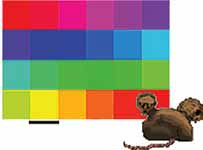
\includegraphics[width=0.8\textwidth]{99_images/keck-1-1a}%chktex 8
    \end{column}
    \begin{column}{0.5\textwidth}
      \centering
      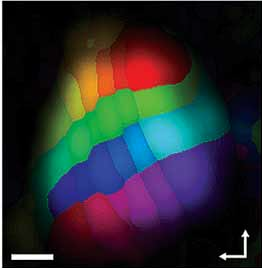
\includegraphics[width=0.8\textwidth]{99_images/keck-1-1c}%chktex 8
    \end{column}
  \end{columns}
  \footnotetext[1]{\fullcite{Keck2008}}
\end{frame}
\begin{frame}[c]{Experimental protocol II:\ after peripheral lesion}
  \note[item]{Then, a part of the retina is lesioned. This cuts off inputs to a part of the visual cortex, as shown in the first figure. This forms the Lesion Projection Zone (LPZ). By repeated imaging of the region over months, the reorganisation of the network is tracked.}
  \note[item]{Other lesion studies use similar methods: digit removal, whisker trimming, and so on---anything that cuts off projecting activity on to a set of neurons.}
    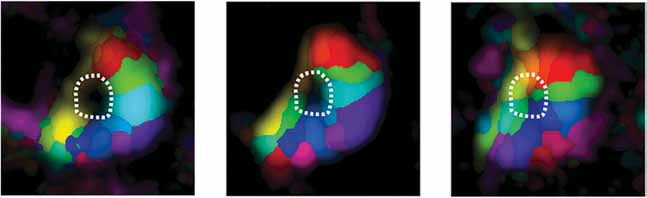
\includegraphics[width=\textwidth]{99_images/keck-1-2c}%chktex 8
    \footnotetext[1]{\fullcite{Keck2008}}
\end{frame}
\begin{frame}[c]{What we know from these experiments}
  \note[item]{So, if this a simple schematic, of the regions around the LPZ, this is what we know from these studies.}
  \begin{columns}
    \begin{column}{0.3\textwidth}
      \centering
      \def\radiuscircle{0.6cm}
\begin{tikzpicture}[scale=0.8, transform shape]
  \fill [fill=black, thick, opacity=0.10] (0,0) rectangle ++(5,7.5);
  \node [below, black] at (3.5, 1.0){Other};

  \fill [cyan, opacity=1.0] (2.5, 3.5) circle (3.0*\radiuscircle);
  \draw [cyan, very thick] (1.5, 1.0)--(2.5, 3.5);
  \node [below, cyan] at (1.5, 1.0){Peri LPZ};

  \fill [black, opacity=1.0] (2.5, 3.5) circle (2.0*\radiuscircle);
  \draw [black, very thick] (1.5, 6.0)--(2.5, 3.5);
  \node [above, black] at (1.5, 6.0){LPZ B};

  \fill [green, opacity=1.0] (2.5, 3.5) circle (\radiuscircle);
  \draw [green, very thick] (3.5, 6.0)--(2.5, 3.5);
  \node [above, green] at (3.5, 6.0){LPZ C};

\end{tikzpicture}

    \end{column}
    \pause{}
    \begin{column}{0.6\textwidth}
      \begin{itemize}
        \item Massive disinhibition in the LPZ\@.
          \note[item]{To permit a window for structural re-organisation.}
        \item Gradual ingrowth of excitatory synapses from the peri-LPZ to the LPZ\@.
          \note[item]{To make up for lost excitation.}
        \item Gradual outgrowth of inhibitory synapses from the LPZ to the peri-LPZ\@.
          \note[item]{To make up for lost inhibition.}
      \end{itemize}
    \end{column}
  \end{columns}
\end{frame}
\begin{frame}[c]{Computational modelling:\ MSP:\ growth curve}
  \note[item]{In the paper, we simply cite this bit and discuss it briefly, but here I'll explain it in more detail here.}
  \note[item]{Computational modelling stems from evidence from decades years ago. It was established that outgrowth depends on the change in the Calcium concentration in neurons.}
  \note[item]{So, in this figure, we see that a neurotransmitter causes a change in the Calcium of the neuron, and that causes some change in its outgrowth.}
  \note[item]{What this suggests, is that there's an optimal level of Calcium for neurons to have \enquote{normal} growth.}
  \note[item]{Based on this, Butz and van Ooyen came up with a framework for modelling structural plasticity. In this, they modelled the rate of change of synaptic elements as a Gaussian function of the neuron's Calcium concentration.}
  \begin{columns}
    \begin{column}{0.5\textwidth}
      \centering
      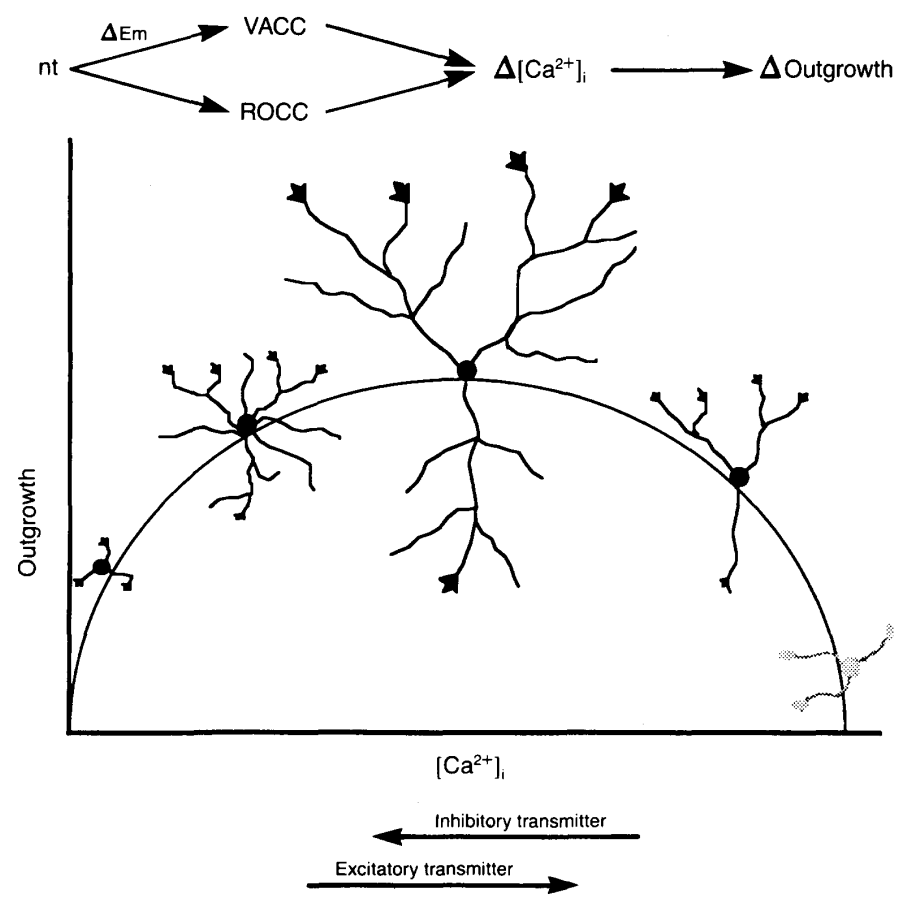
\includegraphics[width=0.9\textwidth]{99_images/lipton1989.png}%chktex 8
    \end{column}
    \begin{column}{0.5\textwidth}
      \centering
      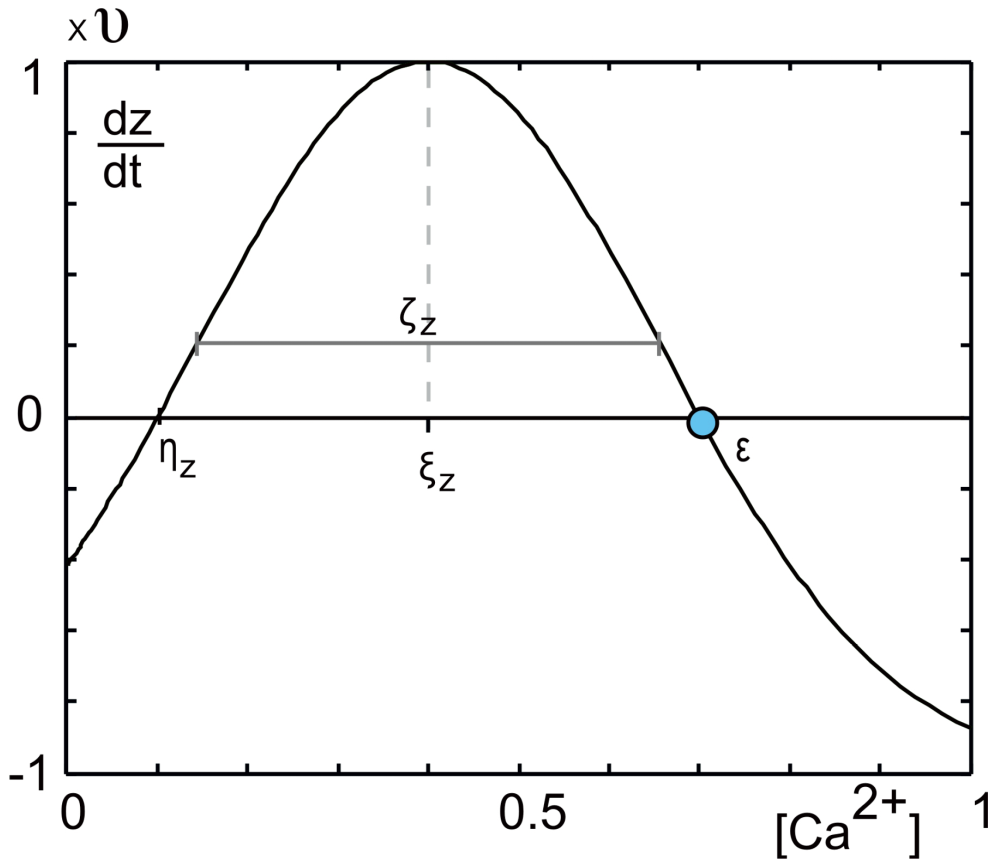
\includegraphics[width=0.9\textwidth]{99_images/growth-curve-general.png}%chktex 8
    \end{column}
  \end{columns}
  \footnotetext[2]{\fullcite{Lipton1989}}
  \footnotetext[3]{\fullcite{Butz2013}}
\end{frame}
\begin{frame}[c]{Computational modelling:\ MSP:\ turnover}
  \note[item]{A stable fixed point where nothing occurs. If activity is less, sprouting, if more, retraction, but if very less, retraction}.
  \note[item]{Note that they applied the same for excitatory and inhibitory post-synaptic elements}
  \note[item]{And, the same for all neurons: excitatory and inhibitory.}
  \begin{columns}
    \begin{column}{0.6\textwidth}
      \begin{itemize}
        \item Synaptic structures (\(z\)): excitatory \alert{and} inhibitory post-synaptic, excitatory \alert{or} inhibitory pre-synaptic elements.
        \item New synapses form when \alert{free} plugs are available: (\(z > z_{conn}\))
        \item Synapses are deleted if: (\(z < z_{conn}\))
      \end{itemize}
    \end{column}
    \begin{column}{0.5\textwidth}
      \centering
      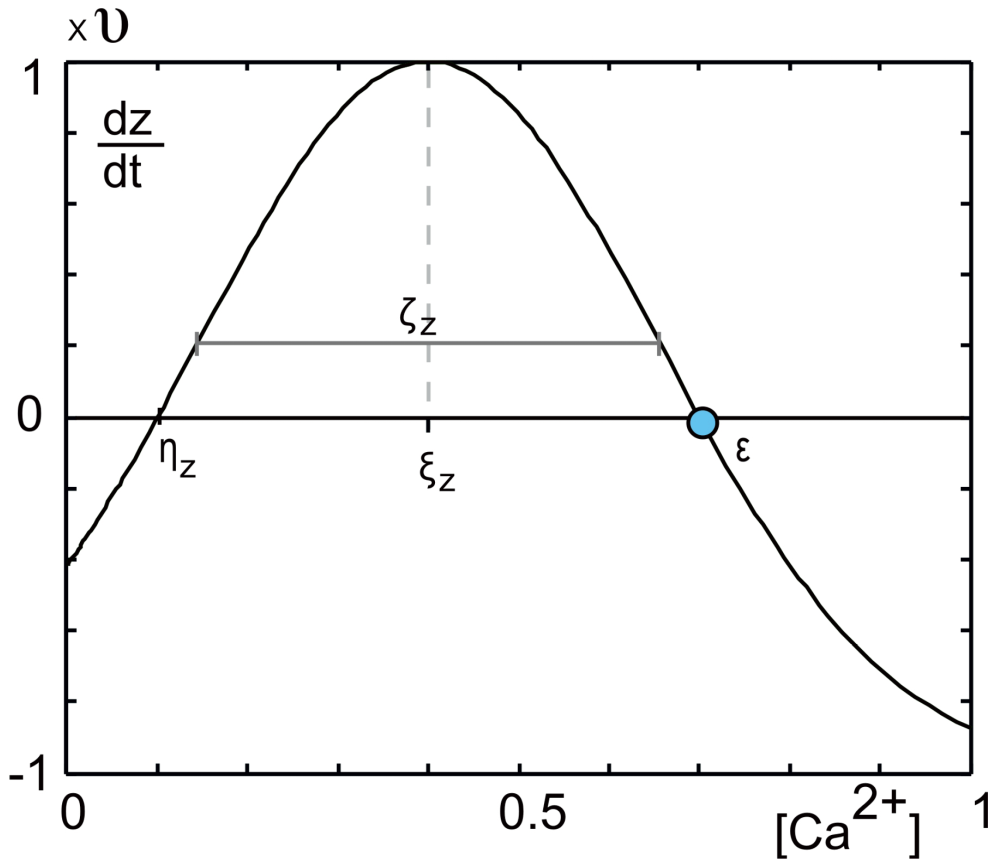
\includegraphics[width=0.9\textwidth]{99_images/growth-curve-general.png}%chktex 8
    \end{column}
  \end{columns}
\end{frame}
\begin{frame}[c]{Computational modelling II:\ Butz2013 replication}
  \centering
  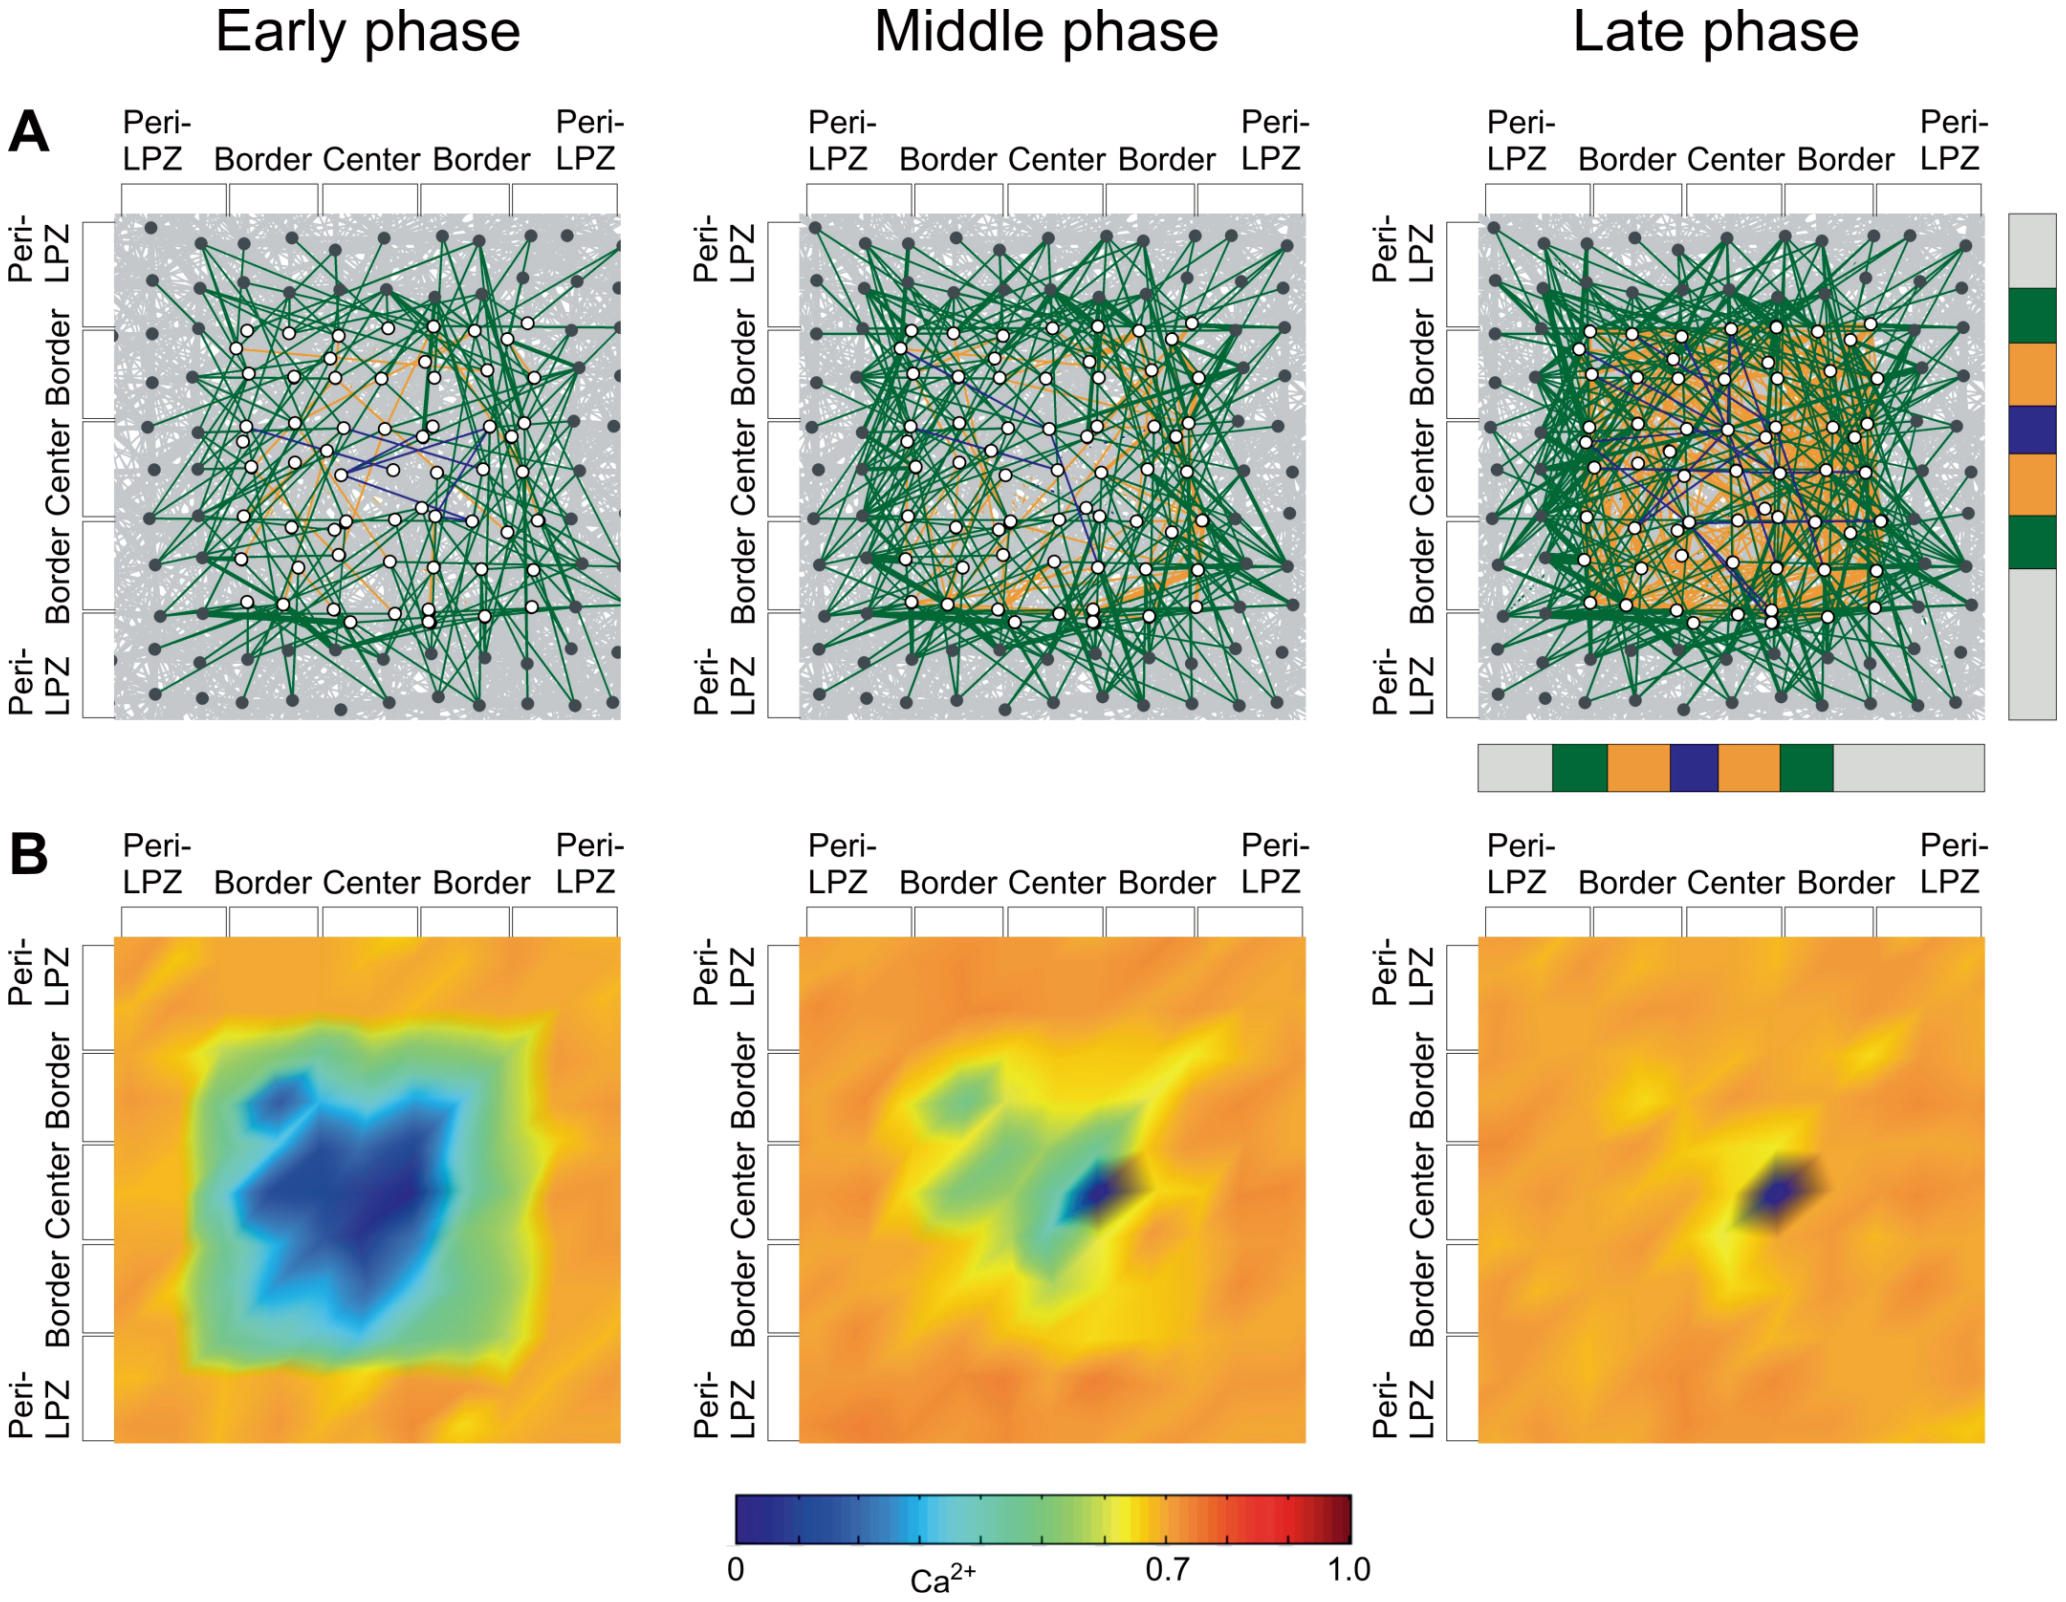
\includegraphics[width=0.9\textwidth]{99_images/butz3.png}
  \note[item]{They replicated the peripheral lesion study, as you see.}
  \note[item]{You have repair from the outside in, and you have ingrowth of excitatory axons.}
\end{frame}
\begin{frame}[c]{Computational modelling II:\ Butz2013 results}
  \begin{columns}
    \begin{column}{0.5\textwidth}
      \begin{figure}[h]
        \begin{tikzpicture}[scale=1, transform shape]
  \begin{axis}[
    no markers, domain=-0:10, samples=100,
    y label style={rotate=-90},
    axis line style={->},
    axis lines*=left, xlabel={\([Ca^{2+}]\)}, ylabel={},
    grid=major, ytick={0}, xtick=\empty, clip=false,
    % axis on top,
    height=5cm, width=\textwidth, enlargelimits=false
    ]
    \addplot [thick, green] {gaussnew(1,1.0, 7.0, 1.0)};
    \addplot [thick, blue] {gaussnew(1,4.0, 7.0, 1.0)};


    \node[left] (A) at (axis cs:0.0, 1){\(\nu\)};
    \node[left] (B) at (axis cs:0.0, -1){\(-\nu\)};
    \node[below] at (axis cs:1., 0.0000){\(\eta_{post}\)};
    \node[below] at (axis cs:4., 0.0000){\(\eta_{pre}\)};
    \node[below right] at (axis cs:7., 0.0000){\(\epsilon\)};
  \end{axis}
\end{tikzpicture}

      \end{figure}
    \end{column}
    \begin{column}{0.5\textwidth}
      \centering
      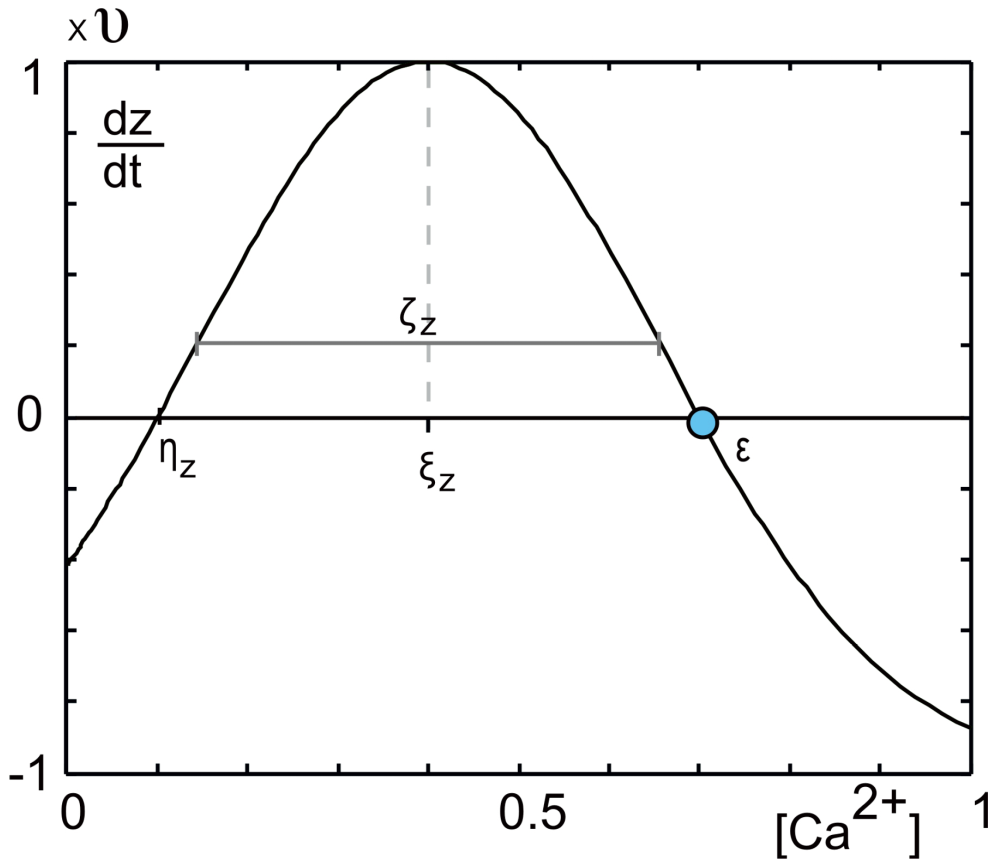
\includegraphics[width=0.9\textwidth]{99_images/growth-curve-general.png}%chktex 8
    \end{column}
  \end{columns}
  \note[item]{They suggested that post-synaptic elements should form at a lower activity level than pre-synaptic elements}
  \note[item]{They used an arbitrary homeostatic point, for all neurons}
  \note[item]{No discussion of inhibitory circuit here.}
  \note[item]{No discussion of biological realism of the model either.}
\end{frame}
\section{Methods: our approach}
\begin{frame}[c]{Start with a biologically realistic network model}
  \begin{figure}[h]
    \def\svgwidth{0.7\textwidth}
    %% Creator: Inkscape inkscape 0.92+devel, www.inkscape.org
%% PDF/EPS/PS + LaTeX output extension by Johan Engelen, 2010
%% Accompanies image file 'schematic.eps' (pdf, eps, ps)
%%
%% To include the image in your LaTeX document, write
%%   \input{<filename>.pdf_tex}
%%  instead of
%%   \includegraphics{<filename>.pdf}
%% To scale the image, write
%%   \def\svgwidth{<desired width>}
%%   \input{<filename>.pdf_tex}
%%  instead of
%%   \includegraphics[width=<desired width>]{<filename>.pdf}
%%
%% Images with a different path to the parent latex file can
%% be accessed with the `import' package (which may need to be
%% installed) using
%%   \usepackage{import}
%% in the preamble, and then including the image with
%%   \import{<path to file>}{<filename>.pdf_tex}
%% Alternatively, one can specify
%%   \graphicspath{{<path to file>/}}
%% 
%% For more information, please see info/svg-inkscape on CTAN:
%%   http://tug.ctan.org/tex-archive/info/svg-inkscape
%%
\begingroup%
  \makeatletter%
  \providecommand\color[2][]{%
    \errmessage{(Inkscape) Color is used for the text in Inkscape, but the package `color.sty' is not loaded}%
    \renewcommand\color[2][]{}%
  }%
  \providecommand\transparent[1]{%
    \errmessage{(Inkscape) Transparency is used (non-zero) for the text in Inkscape, but the package `transparent.sty' is not loaded}%
    \renewcommand\transparent[1]{}%
  }%
  \providecommand\rotatebox[2]{#2}%
  \ifx\svgwidth\undefined%
    \setlength{\unitlength}{841.88976378bp}%
    \ifx\svgscale\undefined%
      \relax%
    \else%
      \setlength{\unitlength}{\unitlength{} * \real{\svgscale}}%
    \fi%
  \else%
    \setlength{\unitlength}{\svgwidth}%
  \fi%
  \global\let\svgwidth\undefined%
  \global\let\svgscale\undefined%
  \makeatother%
  \begin{picture}(1,0.8)(0,-0.1)%
    \put(0,0.05){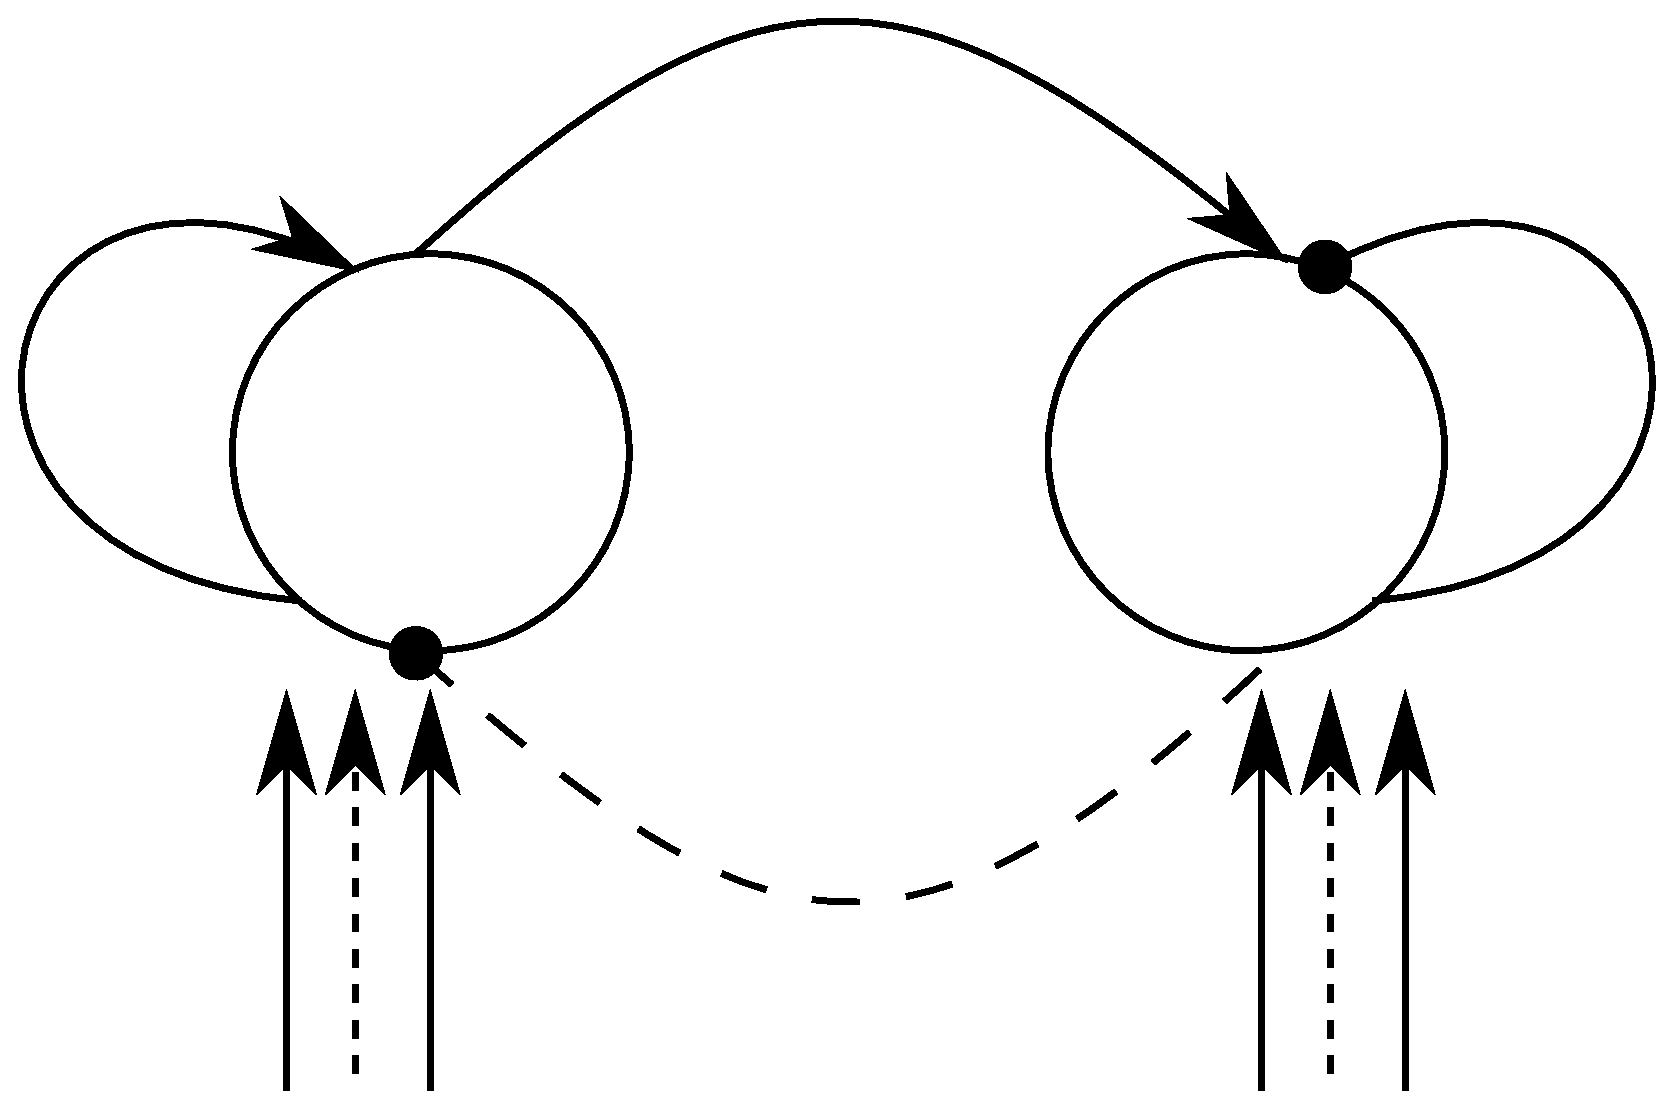
\includegraphics[width=\unitlength]{99_images/schematic.eps}}%
    \put(0.2347176,0.44870591){\color[rgb]{0,0,0}\makebox(0,0)[lb]{\smash{E}}}%
    \put(0.1747176,0.40870591){\color[rgb]{0,0,0}\makebox(0,0)[lb]{\smash{neurons}}}%
    \put(0.73973984,0.44870591){\color[rgb]{0,0,0}\makebox(0,0)[lb]{\smash{I}}}%
    \put(0.66973984,0.40870591){\color[rgb]{0,0,0}\makebox(0,0)[lb]{\smash{neurons}}}%
    \put(0.00355224,0.58941411){\color[rgb]{0,0,0}\makebox(0,0)[lb]{\smash{\(g_{EE}\)}}}%
    \put(0.46685226,0.65011583){\color[rgb]{0,0,0}\makebox(0,0)[lb]{\smash{\(g_{EI}\)}}}%
    \put(0.94063961,0.58941411){\color[rgb]{0,0,0}\makebox(0,0)[lb]{\smash{\(g_{II}\)}}}%
    \put(0.45717629,0.09520415){\color[rgb]{0,0,0}\makebox(0,0)[lb]{\smash{\(g_{IE}\)}}}%
    \put(0.05,0.09520415){\color[rgb]{0,0,0}\makebox(0,0)[lb]{\smash{\(g_{ext}^E\)}}}%
    \put(0.86,0.09520415){\color[rgb]{0,0,0}\makebox(0,0)[lb]{\smash{\(g_{ext}^I\)}}}%
    \put(0.08028497,0.00){\color[rgb]{0,0,0}\makebox(0,0)[lb]{\smash{Ext stimulus}}}%
    \put(0.68617882,0.00){\color[rgb]{0,0,0}\makebox(0,0)[lb]{\smash{Ext stimulus}}}%
  \end{picture}%
\endgroup%


  \end{figure}
  \note[item]{We decided to start with a biologically realistic model: a cortical model proposed by Vogels et al.}
  \note[item]{This includes realistic conductances, for example.}
  \note[item]{This model is balanced by homeostatic inhibitory synaptic plasticity, and exhibits AI characteristics similar to cortical networks}
  \note[item]{This model does not have any spatial information incorporated it, but to model the LPZ and spatial analysis we do need it.}
  \footnotetext[4]{\fullcite{Vogels2011}}
\end{frame}
\begin{frame}[c]{Extensions}
  \note[item]{A few of these were made while incorporating spatial information in the model, keeping in mind that we want' to keep the model as realistica as we can manage.}
  \begin{itemize}
    \item Probabilistic formation of synapses, also: \enquote{longer} inhibitory than excitatory connections\footnotemark{}.
    \item Probabilistic deletion of synapses (incorporating evidence that stronger synapses have less likelihood of removal\footnotemark{}).
    \item Further generalisation of growth curves.
  \end{itemize}
  \footnotetext[5]{Citation buried in my lab logs somewhere!}
  \footnotetext[6]{\fullcite{Knott2006}}
\end{frame}
\begin{frame}[c]{Simulation protocol}
  \begin{figure}[h]
    \centering
    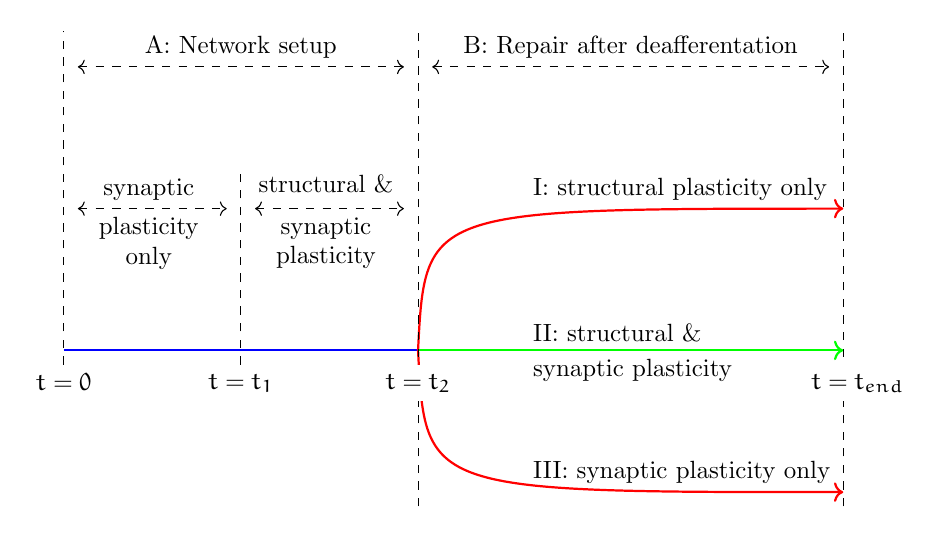
\begin{tikzpicture}[scale=0.9, transform shape]

  % horizontal lines
  \draw[blue, thick] (0,4) -- (5,4);
  \draw[green, thick, ->] (5,4) -- (11,4);
  \draw[red, thick, ->] (5,4) .. controls (5.1,6) .. (11,6);
  \draw[red, thick, ->] (5,4) .. controls (5.1,2) .. (11,2);


  \draw[dashed] (0,3.8) -- (0,8.5);
  \node[below] at (0, 3.8)  {\(t=0\)};

  \draw[dashed] (2.5,3.8) -- (2.5,6.5);
  \node[below] at (2.5, 3.8)  {\(t=t_1\)};

  \draw[dashed, -] (5,1.8) -- (5,8.5);
  \node[below, fill=white] at (5, 3.8)  {\(t=t_2\)};

  \draw[dashed] (11,1.8) -- (11,8.5);
  \node[below, fill=white] at (11.2, 3.8)  {\(t=t_{end}\)};

  \draw[dashed, <->] (0.2,8) -- (4.8,8);
  \node[above] at (2.5,8) {A: Network setup};

  \draw[dashed, <->] (0.2,6) -- (2.3,6);
  \node[above] at (1.2,6) {synaptic};
  \node[below, align=center] at (1.2,6) {plasticity\\only};
  \draw[dashed, <->] (2.7,6) -- (4.8,6);
  \node[above] at (3.7,6.1) {structural \&};
  \node[below, align=center] at (3.7,6) {synaptic\\plasticity};

  \draw[dashed, <->] (5.2,8) -- (10.8,8);
  \node[above] at (8,8) {B: Repair after deafferentation};


  \node[above right, align=left] at (6.5,6) {I: structural plasticity only};
  \node[above right, align=left] at (6.5,4) {II: structural \&};
  \node[below right, align=left] at (6.5,4) {synaptic plasticity};
  \node[above right, align=left] at (6.5,2) {III: synaptic plasticity only};

\end{tikzpicture}

  \end{figure}
  \note[item]{Explain the simulation protocol.}
\end{frame}
\section{Results and discussion}
\begin{frame}[c]{Deafferentation and successful repair}
  \begin{figure}
      \centering
      \resizebox{\textwidth}{!}{% GNUPLOT: LaTeX picture with Postscript
\begingroup
  \makeatletter
  \providecommand\color[2][]{%
    \GenericError{(gnuplot) \space\space\space\@spaces}{%
      Package color not loaded in conjunction with
      terminal option `colourtext'%
    }{See the gnuplot documentation for explanation.%
    }{Either use 'blacktext' in gnuplot or load the package
      color.sty in LaTeX.}%
    \renewcommand\color[2][]{}%
  }%
  \providecommand\includegraphics[2][]{%
    \GenericError{(gnuplot) \space\space\space\@spaces}{%
      Package graphicx or graphics not loaded%
    }{See the gnuplot documentation for explanation.%
    }{The gnuplot epslatex terminal needs graphicx.sty or graphics.sty.}%
    \renewcommand\includegraphics[2][]{}%
  }%
  \providecommand\rotatebox[2]{#2}%
  \@ifundefined{ifGPcolor}{%
    \newif\ifGPcolor
    \GPcolortrue
  }{}%
  \@ifundefined{ifGPblacktext}{%
    \newif\ifGPblacktext
    \GPblacktexttrue
  }{}%
  % define a \g@addto@macro without @ in the name:
  \let\gplgaddtomacro\g@addto@macro
  % define empty templates for all commands taking text:
  \gdef\gplbacktext{}%
  \gdef\gplfronttext{}%
  \makeatother
  \ifGPblacktext
    % no textcolor at all
    \def\colorrgb#1{}%
    \def\colorgray#1{}%
  \else
    % gray or color?
    \ifGPcolor
      \def\colorrgb#1{\color[rgb]{#1}}%
      \def\colorgray#1{\color[gray]{#1}}%
      \expandafter\def\csname LTw\endcsname{\color{white}}%
      \expandafter\def\csname LTb\endcsname{\color{black}}%
      \expandafter\def\csname LTa\endcsname{\color{black}}%
      \expandafter\def\csname LT0\endcsname{\color[rgb]{1,0,0}}%
      \expandafter\def\csname LT1\endcsname{\color[rgb]{0,1,0}}%
      \expandafter\def\csname LT2\endcsname{\color[rgb]{0,0,1}}%
      \expandafter\def\csname LT3\endcsname{\color[rgb]{1,0,1}}%
      \expandafter\def\csname LT4\endcsname{\color[rgb]{0,1,1}}%
      \expandafter\def\csname LT5\endcsname{\color[rgb]{1,1,0}}%
      \expandafter\def\csname LT6\endcsname{\color[rgb]{0,0,0}}%
      \expandafter\def\csname LT7\endcsname{\color[rgb]{1,0.3,0}}%
      \expandafter\def\csname LT8\endcsname{\color[rgb]{0.5,0.5,0.5}}%
    \else
      % gray
      \def\colorrgb#1{\color{black}}%
      \def\colorgray#1{\color[gray]{#1}}%
      \expandafter\def\csname LTw\endcsname{\color{white}}%
      \expandafter\def\csname LTb\endcsname{\color{black}}%
      \expandafter\def\csname LTa\endcsname{\color{black}}%
      \expandafter\def\csname LT0\endcsname{\color{black}}%
      \expandafter\def\csname LT1\endcsname{\color{black}}%
      \expandafter\def\csname LT2\endcsname{\color{black}}%
      \expandafter\def\csname LT3\endcsname{\color{black}}%
      \expandafter\def\csname LT4\endcsname{\color{black}}%
      \expandafter\def\csname LT5\endcsname{\color{black}}%
      \expandafter\def\csname LT6\endcsname{\color{black}}%
      \expandafter\def\csname LT7\endcsname{\color{black}}%
      \expandafter\def\csname LT8\endcsname{\color{black}}%
    \fi
  \fi
    \setlength{\unitlength}{0.0500bp}%
    \ifx\gptboxheight\undefined%
      \newlength{\gptboxheight}%
      \newlength{\gptboxwidth}%
      \newsavebox{\gptboxtext}%
    \fi%
    \setlength{\fboxrule}{0.5pt}%
    \setlength{\fboxsep}{1pt}%
\begin{picture}(7936.00,2550.00)%
    \gplgaddtomacro\gplbacktext{%
    }%
    \gplgaddtomacro\gplfronttext{%
    }%
    \gplgaddtomacro\gplbacktext{%
    }%
    \gplgaddtomacro\gplfronttext{%
    }%
    \gplgaddtomacro\gplbacktext{%
    }%
    \gplgaddtomacro\gplfronttext{%
    }%
    \gplgaddtomacro\gplbacktext{%
    }%
    \gplgaddtomacro\gplfronttext{%
      \csname LTb\endcsname%
      \put(7554,51){\makebox(0,0)[l]{\strut{}$1$}}%
      \put(7554,2285){\makebox(0,0)[l]{\strut{}$5$}}%
      \put(7752,1168){\rotatebox{-270}{\makebox(0,0){\strut{}Firing rate (Hz)}}}%
    }%
    \gplbacktext
    \put(0,0){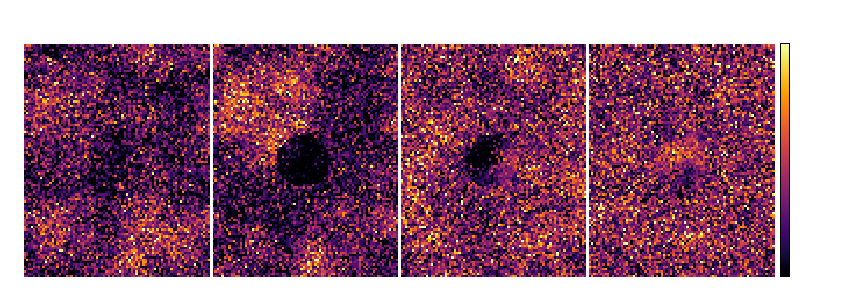
\includegraphics[interpolate=false]{99_images/201811221433-firing-rate-snapshots-E}}%
    \gplfronttext
  \end{picture}%
\endgroup
}%
  \end{figure}
\end{frame}
\begin{frame}[c]{Deafferentation and repair:\ LPZ}
  \begin{figure}
      \centering
      \resizebox{\textwidth}{!}{% GNUPLOT: LaTeX picture with Postscript
\begingroup
  \makeatletter
  \providecommand\color[2][]{%
    \GenericError{(gnuplot) \space\space\space\@spaces}{%
      Package color not loaded in conjunction with
      terminal option `colourtext'%
    }{See the gnuplot documentation for explanation.%
    }{Either use 'blacktext' in gnuplot or load the package
      color.sty in LaTeX.}%
    \renewcommand\color[2][]{}%
  }%
  \providecommand\includegraphics[2][]{%
    \GenericError{(gnuplot) \space\space\space\@spaces}{%
      Package graphicx or graphics not loaded%
    }{See the gnuplot documentation for explanation.%
    }{The gnuplot epslatex terminal needs graphicx.sty or graphics.sty.}%
    \renewcommand\includegraphics[2][]{}%
  }%
  \providecommand\rotatebox[2]{#2}%
  \@ifundefined{ifGPcolor}{%
    \newif\ifGPcolor
    \GPcolortrue
  }{}%
  \@ifundefined{ifGPblacktext}{%
    \newif\ifGPblacktext
    \GPblacktexttrue
  }{}%
  % define a \g@addto@macro without @ in the name:
  \let\gplgaddtomacro\g@addto@macro
  % define empty templates for all commands taking text:
  \gdef\gplbacktext{}%
  \gdef\gplfronttext{}%
  \makeatother
  \ifGPblacktext
    % no textcolor at all
    \def\colorrgb#1{}%
    \def\colorgray#1{}%
  \else
    % gray or color?
    \ifGPcolor
      \def\colorrgb#1{\color[rgb]{#1}}%
      \def\colorgray#1{\color[gray]{#1}}%
      \expandafter\def\csname LTw\endcsname{\color{white}}%
      \expandafter\def\csname LTb\endcsname{\color{black}}%
      \expandafter\def\csname LTa\endcsname{\color{black}}%
      \expandafter\def\csname LT0\endcsname{\color[rgb]{1,0,0}}%
      \expandafter\def\csname LT1\endcsname{\color[rgb]{0,1,0}}%
      \expandafter\def\csname LT2\endcsname{\color[rgb]{0,0,1}}%
      \expandafter\def\csname LT3\endcsname{\color[rgb]{1,0,1}}%
      \expandafter\def\csname LT4\endcsname{\color[rgb]{0,1,1}}%
      \expandafter\def\csname LT5\endcsname{\color[rgb]{1,1,0}}%
      \expandafter\def\csname LT6\endcsname{\color[rgb]{0,0,0}}%
      \expandafter\def\csname LT7\endcsname{\color[rgb]{1,0.3,0}}%
      \expandafter\def\csname LT8\endcsname{\color[rgb]{0.5,0.5,0.5}}%
    \else
      % gray
      \def\colorrgb#1{\color{black}}%
      \def\colorgray#1{\color[gray]{#1}}%
      \expandafter\def\csname LTw\endcsname{\color{white}}%
      \expandafter\def\csname LTb\endcsname{\color{black}}%
      \expandafter\def\csname LTa\endcsname{\color{black}}%
      \expandafter\def\csname LT0\endcsname{\color{black}}%
      \expandafter\def\csname LT1\endcsname{\color{black}}%
      \expandafter\def\csname LT2\endcsname{\color{black}}%
      \expandafter\def\csname LT3\endcsname{\color{black}}%
      \expandafter\def\csname LT4\endcsname{\color{black}}%
      \expandafter\def\csname LT5\endcsname{\color{black}}%
      \expandafter\def\csname LT6\endcsname{\color{black}}%
      \expandafter\def\csname LT7\endcsname{\color{black}}%
      \expandafter\def\csname LT8\endcsname{\color{black}}%
    \fi
  \fi
    \setlength{\unitlength}{0.0500bp}%
    \ifx\gptboxheight\undefined%
      \newlength{\gptboxheight}%
      \newlength{\gptboxwidth}%
      \newsavebox{\gptboxtext}%
    \fi%
    \setlength{\fboxrule}{0.5pt}%
    \setlength{\fboxsep}{1pt}%
\begin{picture}(7200.00,2160.00)%
    \gplgaddtomacro\gplbacktext{%
      \csname LTb\endcsname%
      \put(-60,704){\makebox(0,0)[r]{\strut{}$0$}}%
      \put(-60,1101){\makebox(0,0)[r]{\strut{}$2$}}%
      \put(-60,1498){\makebox(0,0)[r]{\strut{}$4$}}%
      \put(-60,1895){\makebox(0,0)[r]{\strut{}$6$}}%
      \put(72,484){\makebox(0,0){\strut{}$0$}}%
      \put(1034,484){\makebox(0,0){\strut{}$1000$}}%
      \put(1995,484){\makebox(0,0){\strut{}$2000$}}%
      \put(2957,484){\makebox(0,0){\strut{}$3000$}}%
      \put(3918,484){\makebox(0,0){\strut{}$4000$}}%
      \put(4880,484){\makebox(0,0){\strut{}$5000$}}%
      \put(5841,484){\makebox(0,0){\strut{}$6000$}}%
      \put(6803,484){\makebox(0,0){\strut{}$7000$}}%
    }%
    \gplgaddtomacro\gplfronttext{%
      \csname LTb\endcsname%
      \put(-434,1299){\rotatebox{-270}{\makebox(0,0){\strut{}Firing rate (Hz)}}}%
      \put(3437,154){\makebox(0,0){\strut{}Time (\(s\))}}%
      \put(3437,1785){\makebox(0,0){\strut{}}}%
      \csname LTb\endcsname%
      \put(5816,1722){\makebox(0,0)[r]{\strut{}I}}%
      \csname LTb\endcsname%
      \put(5816,1502){\makebox(0,0)[r]{\strut{}E}}%
    }%
    \gplbacktext
    \put(0,0){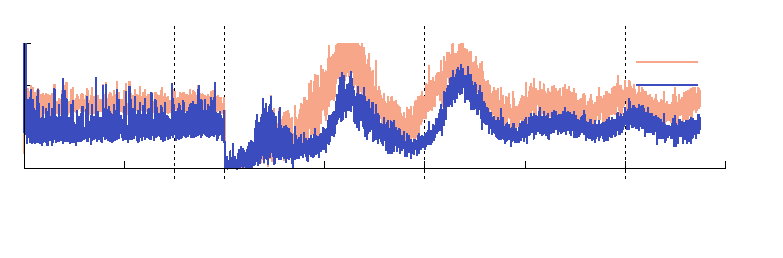
\includegraphics{99_images/201811221433-mean-firing-rates-lpz_c_I-E-zoomed}}%
    \gplfronttext
  \end{picture}%
\endgroup
}%
  \end{figure}
\end{frame}
\begin{frame}[c]{Deafferentation and repair:\ outside the LPZ}
  \note[item]{This is something different now: the activity outside the LPZ goes up after deafferentation}
  \note[item]{First indication that previous models werent thorough enough.}
  \begin{figure}
      \centering
      \resizebox{\textwidth}{!}{% GNUPLOT: LaTeX picture with Postscript
\begingroup
  \makeatletter
  \providecommand\color[2][]{%
    \GenericError{(gnuplot) \space\space\space\@spaces}{%
      Package color not loaded in conjunction with
      terminal option `colourtext'%
    }{See the gnuplot documentation for explanation.%
    }{Either use 'blacktext' in gnuplot or load the package
      color.sty in LaTeX.}%
    \renewcommand\color[2][]{}%
  }%
  \providecommand\includegraphics[2][]{%
    \GenericError{(gnuplot) \space\space\space\@spaces}{%
      Package graphicx or graphics not loaded%
    }{See the gnuplot documentation for explanation.%
    }{The gnuplot epslatex terminal needs graphicx.sty or graphics.sty.}%
    \renewcommand\includegraphics[2][]{}%
  }%
  \providecommand\rotatebox[2]{#2}%
  \@ifundefined{ifGPcolor}{%
    \newif\ifGPcolor
    \GPcolortrue
  }{}%
  \@ifundefined{ifGPblacktext}{%
    \newif\ifGPblacktext
    \GPblacktexttrue
  }{}%
  % define a \g@addto@macro without @ in the name:
  \let\gplgaddtomacro\g@addto@macro
  % define empty templates for all commands taking text:
  \gdef\gplbacktext{}%
  \gdef\gplfronttext{}%
  \makeatother
  \ifGPblacktext
    % no textcolor at all
    \def\colorrgb#1{}%
    \def\colorgray#1{}%
  \else
    % gray or color?
    \ifGPcolor
      \def\colorrgb#1{\color[rgb]{#1}}%
      \def\colorgray#1{\color[gray]{#1}}%
      \expandafter\def\csname LTw\endcsname{\color{white}}%
      \expandafter\def\csname LTb\endcsname{\color{black}}%
      \expandafter\def\csname LTa\endcsname{\color{black}}%
      \expandafter\def\csname LT0\endcsname{\color[rgb]{1,0,0}}%
      \expandafter\def\csname LT1\endcsname{\color[rgb]{0,1,0}}%
      \expandafter\def\csname LT2\endcsname{\color[rgb]{0,0,1}}%
      \expandafter\def\csname LT3\endcsname{\color[rgb]{1,0,1}}%
      \expandafter\def\csname LT4\endcsname{\color[rgb]{0,1,1}}%
      \expandafter\def\csname LT5\endcsname{\color[rgb]{1,1,0}}%
      \expandafter\def\csname LT6\endcsname{\color[rgb]{0,0,0}}%
      \expandafter\def\csname LT7\endcsname{\color[rgb]{1,0.3,0}}%
      \expandafter\def\csname LT8\endcsname{\color[rgb]{0.5,0.5,0.5}}%
    \else
      % gray
      \def\colorrgb#1{\color{black}}%
      \def\colorgray#1{\color[gray]{#1}}%
      \expandafter\def\csname LTw\endcsname{\color{white}}%
      \expandafter\def\csname LTb\endcsname{\color{black}}%
      \expandafter\def\csname LTa\endcsname{\color{black}}%
      \expandafter\def\csname LT0\endcsname{\color{black}}%
      \expandafter\def\csname LT1\endcsname{\color{black}}%
      \expandafter\def\csname LT2\endcsname{\color{black}}%
      \expandafter\def\csname LT3\endcsname{\color{black}}%
      \expandafter\def\csname LT4\endcsname{\color{black}}%
      \expandafter\def\csname LT5\endcsname{\color{black}}%
      \expandafter\def\csname LT6\endcsname{\color{black}}%
      \expandafter\def\csname LT7\endcsname{\color{black}}%
      \expandafter\def\csname LT8\endcsname{\color{black}}%
    \fi
  \fi
    \setlength{\unitlength}{0.0500bp}%
    \ifx\gptboxheight\undefined%
      \newlength{\gptboxheight}%
      \newlength{\gptboxwidth}%
      \newsavebox{\gptboxtext}%
    \fi%
    \setlength{\fboxrule}{0.5pt}%
    \setlength{\fboxsep}{1pt}%
\begin{picture}(7200.00,2160.00)%
    \gplgaddtomacro\gplbacktext{%
      \csname LTb\endcsname%
      \put(-60,704){\makebox(0,0)[r]{\strut{}$0$}}%
      \put(-60,1101){\makebox(0,0)[r]{\strut{}$2$}}%
      \put(-60,1498){\makebox(0,0)[r]{\strut{}$4$}}%
      \put(-60,1895){\makebox(0,0)[r]{\strut{}$6$}}%
      \put(72,484){\makebox(0,0){\strut{}$0$}}%
      \put(1034,484){\makebox(0,0){\strut{}$1000$}}%
      \put(1995,484){\makebox(0,0){\strut{}$2000$}}%
      \put(2957,484){\makebox(0,0){\strut{}$3000$}}%
      \put(3918,484){\makebox(0,0){\strut{}$4000$}}%
      \put(4880,484){\makebox(0,0){\strut{}$5000$}}%
      \put(5841,484){\makebox(0,0){\strut{}$6000$}}%
      \put(6803,484){\makebox(0,0){\strut{}$7000$}}%
    }%
    \gplgaddtomacro\gplfronttext{%
      \csname LTb\endcsname%
      \put(-434,1299){\rotatebox{-270}{\makebox(0,0){\strut{}Firing rate (Hz)}}}%
      \put(3437,154){\makebox(0,0){\strut{}Time (\(s\))}}%
      \put(3437,1785){\makebox(0,0){\strut{}}}%
      \csname LTb\endcsname%
      \put(5816,1722){\makebox(0,0)[r]{\strut{}I}}%
      \csname LTb\endcsname%
      \put(5816,1502){\makebox(0,0)[r]{\strut{}E}}%
    }%
    \gplbacktext
    \put(0,0){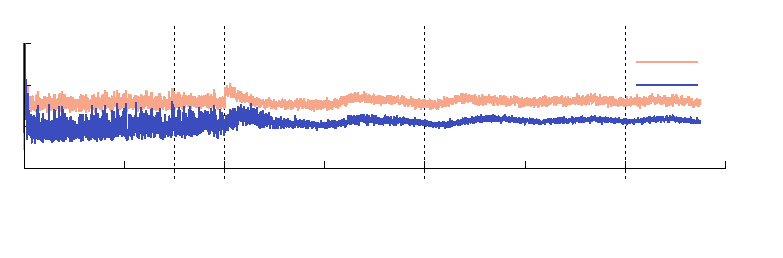
\includegraphics{99_images/201811221433-mean-firing-rates-p_lpz_I-E-zoomed}}%
    \gplfronttext
  \end{picture}%
\endgroup
}%
  \end{figure}
\end{frame}
\begin{frame}[c]{Post-synaptic growth dynamics}
  \begin{columns}
    \begin{column}{0.5\textwidth}
      \begin{figure}[h]
        \begin{tikzpicture}[scale=1, transform shape]
  \begin{axis}[
    no markers, domain=-0:20, samples=100,
    y label style={rotate=-90},
    x axis line style={->},
    y axis line style={<->},
    ymin=-2.0, ymax=3.0,
    axis x line*=center,
    axis y line*=left,
    xlabel={\([Ca^{2+}]\)}, ylabel={\(\frac{dz}{dt}\)},
    grid=major, ytick={0}, xtick=\empty, clip=false,
    axis on top,
    height=6.0cm, width=\textwidth, enlargelimits=false
    ]
    \addplot [thick, blue] {gaussnew(1,5.0, 10.0,1)};
    \addplot [thick, red] {gaussnew(1,10.0, 15.0,1)};

    \draw [thick, dashed, -] (axis cs:10.0, -2.0)--(axis cs:10.0, 2.1);
    \node [above] at (axis cs:10.0, 2.2){\(\psi\)};
    \node [above, blue] at (axis cs:7.5, 2.1){\(z_E\)};
    \node [above, red] at (axis cs:12.5, 2.1){\(z_I\)};

  \end{axis}
\end{tikzpicture}

      \end{figure}
    \end{column}
    \begin{column}{0.6\textwidth}
      \centering
      \begin{itemize}
        \item Loss of activity: sprouting of E, retraction of I
        \item Extra activity: retraction of E, sprouting of I
      \end{itemize}
    \end{column}
  \end{columns}
\end{frame}
\begin{frame}[c]{Resultant turnover:\ LPZ}
  \begin{figure}[t]
    \centering
    \resizebox{0.6\textwidth}{!}{% GNUPLOT: LaTeX picture with Postscript
\begingroup
  \makeatletter
  \providecommand\color[2][]{%
    \GenericError{(gnuplot) \space\space\space\@spaces}{%
      Package color not loaded in conjunction with
      terminal option `colourtext'%
    }{See the gnuplot documentation for explanation.%
    }{Either use 'blacktext' in gnuplot or load the package
      color.sty in LaTeX.}%
    \renewcommand\color[2][]{}%
  }%
  \providecommand\includegraphics[2][]{%
    \GenericError{(gnuplot) \space\space\space\@spaces}{%
      Package graphicx or graphics not loaded%
    }{See the gnuplot documentation for explanation.%
    }{The gnuplot epslatex terminal needs graphicx.sty or graphics.sty.}%
    \renewcommand\includegraphics[2][]{}%
  }%
  \providecommand\rotatebox[2]{#2}%
  \@ifundefined{ifGPcolor}{%
    \newif\ifGPcolor
    \GPcolortrue
  }{}%
  \@ifundefined{ifGPblacktext}{%
    \newif\ifGPblacktext
    \GPblacktexttrue
  }{}%
  % define a \g@addto@macro without @ in the name:
  \let\gplgaddtomacro\g@addto@macro
  % define empty templates for all commands taking text:
  \gdef\gplbacktext{}%
  \gdef\gplfronttext{}%
  \makeatother
  \ifGPblacktext
    % no textcolor at all
    \def\colorrgb#1{}%
    \def\colorgray#1{}%
  \else
    % gray or color?
    \ifGPcolor
      \def\colorrgb#1{\color[rgb]{#1}}%
      \def\colorgray#1{\color[gray]{#1}}%
      \expandafter\def\csname LTw\endcsname{\color{white}}%
      \expandafter\def\csname LTb\endcsname{\color{black}}%
      \expandafter\def\csname LTa\endcsname{\color{black}}%
      \expandafter\def\csname LT0\endcsname{\color[rgb]{1,0,0}}%
      \expandafter\def\csname LT1\endcsname{\color[rgb]{0,1,0}}%
      \expandafter\def\csname LT2\endcsname{\color[rgb]{0,0,1}}%
      \expandafter\def\csname LT3\endcsname{\color[rgb]{1,0,1}}%
      \expandafter\def\csname LT4\endcsname{\color[rgb]{0,1,1}}%
      \expandafter\def\csname LT5\endcsname{\color[rgb]{1,1,0}}%
      \expandafter\def\csname LT6\endcsname{\color[rgb]{0,0,0}}%
      \expandafter\def\csname LT7\endcsname{\color[rgb]{1,0.3,0}}%
      \expandafter\def\csname LT8\endcsname{\color[rgb]{0.5,0.5,0.5}}%
    \else
      % gray
      \def\colorrgb#1{\color{black}}%
      \def\colorgray#1{\color[gray]{#1}}%
      \expandafter\def\csname LTw\endcsname{\color{white}}%
      \expandafter\def\csname LTb\endcsname{\color{black}}%
      \expandafter\def\csname LTa\endcsname{\color{black}}%
      \expandafter\def\csname LT0\endcsname{\color{black}}%
      \expandafter\def\csname LT1\endcsname{\color{black}}%
      \expandafter\def\csname LT2\endcsname{\color{black}}%
      \expandafter\def\csname LT3\endcsname{\color{black}}%
      \expandafter\def\csname LT4\endcsname{\color{black}}%
      \expandafter\def\csname LT5\endcsname{\color{black}}%
      \expandafter\def\csname LT6\endcsname{\color{black}}%
      \expandafter\def\csname LT7\endcsname{\color{black}}%
      \expandafter\def\csname LT8\endcsname{\color{black}}%
    \fi
  \fi
    \setlength{\unitlength}{0.0500bp}%
    \ifx\gptboxheight\undefined%
      \newlength{\gptboxheight}%
      \newlength{\gptboxwidth}%
      \newsavebox{\gptboxtext}%
    \fi%
    \setlength{\fboxrule}{0.5pt}%
    \setlength{\fboxsep}{1pt}%
\begin{picture}(7936.00,2550.00)%
    \gplgaddtomacro\gplbacktext{%
    }%
    \gplgaddtomacro\gplfronttext{%
    }%
    \gplgaddtomacro\gplbacktext{%
    }%
    \gplgaddtomacro\gplfronttext{%
    }%
    \gplgaddtomacro\gplbacktext{%
    }%
    \gplgaddtomacro\gplfronttext{%
    }%
    \gplbacktext
    \put(0,0){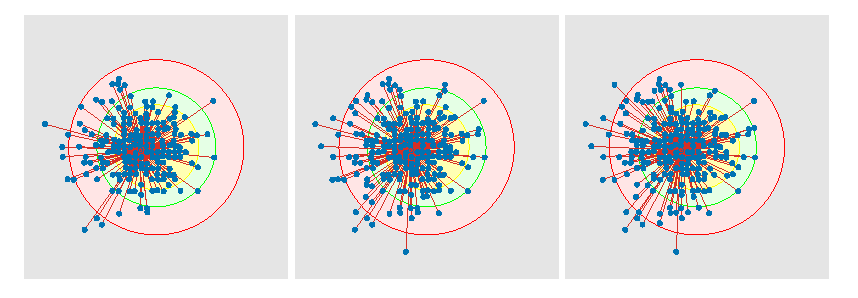
\includegraphics{99_images/201811221433-75-conns-top-EE-lpz_c_E-in}}%
    \gplfronttext
  \end{picture}%
\endgroup
}\\%
    \resizebox{0.6\textwidth}{!}{% GNUPLOT: LaTeX picture with Postscript
\begingroup
  \makeatletter
  \providecommand\color[2][]{%
    \GenericError{(gnuplot) \space\space\space\@spaces}{%
      Package color not loaded in conjunction with
      terminal option `colourtext'%
    }{See the gnuplot documentation for explanation.%
    }{Either use 'blacktext' in gnuplot or load the package
      color.sty in LaTeX.}%
    \renewcommand\color[2][]{}%
  }%
  \providecommand\includegraphics[2][]{%
    \GenericError{(gnuplot) \space\space\space\@spaces}{%
      Package graphicx or graphics not loaded%
    }{See the gnuplot documentation for explanation.%
    }{The gnuplot epslatex terminal needs graphicx.sty or graphics.sty.}%
    \renewcommand\includegraphics[2][]{}%
  }%
  \providecommand\rotatebox[2]{#2}%
  \@ifundefined{ifGPcolor}{%
    \newif\ifGPcolor
    \GPcolortrue
  }{}%
  \@ifundefined{ifGPblacktext}{%
    \newif\ifGPblacktext
    \GPblacktexttrue
  }{}%
  % define a \g@addto@macro without @ in the name:
  \let\gplgaddtomacro\g@addto@macro
  % define empty templates for all commands taking text:
  \gdef\gplbacktext{}%
  \gdef\gplfronttext{}%
  \makeatother
  \ifGPblacktext
    % no textcolor at all
    \def\colorrgb#1{}%
    \def\colorgray#1{}%
  \else
    % gray or color?
    \ifGPcolor
      \def\colorrgb#1{\color[rgb]{#1}}%
      \def\colorgray#1{\color[gray]{#1}}%
      \expandafter\def\csname LTw\endcsname{\color{white}}%
      \expandafter\def\csname LTb\endcsname{\color{black}}%
      \expandafter\def\csname LTa\endcsname{\color{black}}%
      \expandafter\def\csname LT0\endcsname{\color[rgb]{1,0,0}}%
      \expandafter\def\csname LT1\endcsname{\color[rgb]{0,1,0}}%
      \expandafter\def\csname LT2\endcsname{\color[rgb]{0,0,1}}%
      \expandafter\def\csname LT3\endcsname{\color[rgb]{1,0,1}}%
      \expandafter\def\csname LT4\endcsname{\color[rgb]{0,1,1}}%
      \expandafter\def\csname LT5\endcsname{\color[rgb]{1,1,0}}%
      \expandafter\def\csname LT6\endcsname{\color[rgb]{0,0,0}}%
      \expandafter\def\csname LT7\endcsname{\color[rgb]{1,0.3,0}}%
      \expandafter\def\csname LT8\endcsname{\color[rgb]{0.5,0.5,0.5}}%
    \else
      % gray
      \def\colorrgb#1{\color{black}}%
      \def\colorgray#1{\color[gray]{#1}}%
      \expandafter\def\csname LTw\endcsname{\color{white}}%
      \expandafter\def\csname LTb\endcsname{\color{black}}%
      \expandafter\def\csname LTa\endcsname{\color{black}}%
      \expandafter\def\csname LT0\endcsname{\color{black}}%
      \expandafter\def\csname LT1\endcsname{\color{black}}%
      \expandafter\def\csname LT2\endcsname{\color{black}}%
      \expandafter\def\csname LT3\endcsname{\color{black}}%
      \expandafter\def\csname LT4\endcsname{\color{black}}%
      \expandafter\def\csname LT5\endcsname{\color{black}}%
      \expandafter\def\csname LT6\endcsname{\color{black}}%
      \expandafter\def\csname LT7\endcsname{\color{black}}%
      \expandafter\def\csname LT8\endcsname{\color{black}}%
    \fi
  \fi
    \setlength{\unitlength}{0.0500bp}%
    \ifx\gptboxheight\undefined%
      \newlength{\gptboxheight}%
      \newlength{\gptboxwidth}%
      \newsavebox{\gptboxtext}%
    \fi%
    \setlength{\fboxrule}{0.5pt}%
    \setlength{\fboxsep}{1pt}%
\begin{picture}(7936.00,2550.00)%
    \gplgaddtomacro\gplbacktext{%
    }%
    \gplgaddtomacro\gplfronttext{%
    }%
    \gplgaddtomacro\gplbacktext{%
    }%
    \gplgaddtomacro\gplfronttext{%
    }%
    \gplgaddtomacro\gplbacktext{%
    }%
    \gplgaddtomacro\gplfronttext{%
    }%
    \gplbacktext
    \put(0,0){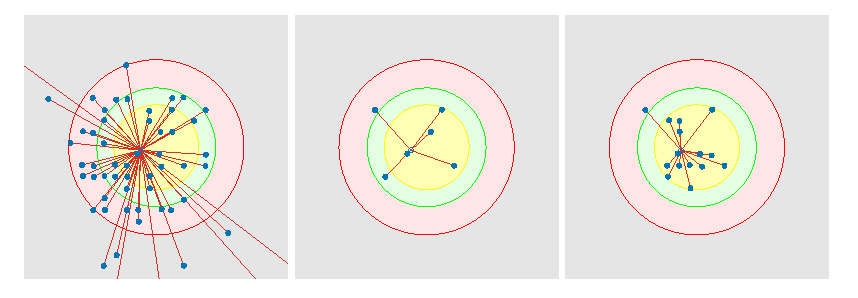
\includegraphics{99_images/201811221433-75-conns-top-IE-lpz_c_E-in}}%
    \gplfronttext
  \end{picture}%
\endgroup
}\\%
    \resizebox{0.6\textwidth}{!}{% GNUPLOT: LaTeX picture with Postscript
\begingroup
  \makeatletter
  \providecommand\color[2][]{%
    \GenericError{(gnuplot) \space\space\space\@spaces}{%
      Package color not loaded in conjunction with
      terminal option `colourtext'%
    }{See the gnuplot documentation for explanation.%
    }{Either use 'blacktext' in gnuplot or load the package
      color.sty in LaTeX.}%
    \renewcommand\color[2][]{}%
  }%
  \providecommand\includegraphics[2][]{%
    \GenericError{(gnuplot) \space\space\space\@spaces}{%
      Package graphicx or graphics not loaded%
    }{See the gnuplot documentation for explanation.%
    }{The gnuplot epslatex terminal needs graphicx.sty or graphics.sty.}%
    \renewcommand\includegraphics[2][]{}%
  }%
  \providecommand\rotatebox[2]{#2}%
  \@ifundefined{ifGPcolor}{%
    \newif\ifGPcolor
    \GPcolortrue
  }{}%
  \@ifundefined{ifGPblacktext}{%
    \newif\ifGPblacktext
    \GPblacktexttrue
  }{}%
  % define a \g@addto@macro without @ in the name:
  \let\gplgaddtomacro\g@addto@macro
  % define empty templates for all commands taking text:
  \gdef\gplbacktext{}%
  \gdef\gplfronttext{}%
  \makeatother
  \ifGPblacktext
    % no textcolor at all
    \def\colorrgb#1{}%
    \def\colorgray#1{}%
  \else
    % gray or color?
    \ifGPcolor
      \def\colorrgb#1{\color[rgb]{#1}}%
      \def\colorgray#1{\color[gray]{#1}}%
      \expandafter\def\csname LTw\endcsname{\color{white}}%
      \expandafter\def\csname LTb\endcsname{\color{black}}%
      \expandafter\def\csname LTa\endcsname{\color{black}}%
      \expandafter\def\csname LT0\endcsname{\color[rgb]{1,0,0}}%
      \expandafter\def\csname LT1\endcsname{\color[rgb]{0,1,0}}%
      \expandafter\def\csname LT2\endcsname{\color[rgb]{0,0,1}}%
      \expandafter\def\csname LT3\endcsname{\color[rgb]{1,0,1}}%
      \expandafter\def\csname LT4\endcsname{\color[rgb]{0,1,1}}%
      \expandafter\def\csname LT5\endcsname{\color[rgb]{1,1,0}}%
      \expandafter\def\csname LT6\endcsname{\color[rgb]{0,0,0}}%
      \expandafter\def\csname LT7\endcsname{\color[rgb]{1,0.3,0}}%
      \expandafter\def\csname LT8\endcsname{\color[rgb]{0.5,0.5,0.5}}%
    \else
      % gray
      \def\colorrgb#1{\color{black}}%
      \def\colorgray#1{\color[gray]{#1}}%
      \expandafter\def\csname LTw\endcsname{\color{white}}%
      \expandafter\def\csname LTb\endcsname{\color{black}}%
      \expandafter\def\csname LTa\endcsname{\color{black}}%
      \expandafter\def\csname LT0\endcsname{\color{black}}%
      \expandafter\def\csname LT1\endcsname{\color{black}}%
      \expandafter\def\csname LT2\endcsname{\color{black}}%
      \expandafter\def\csname LT3\endcsname{\color{black}}%
      \expandafter\def\csname LT4\endcsname{\color{black}}%
      \expandafter\def\csname LT5\endcsname{\color{black}}%
      \expandafter\def\csname LT6\endcsname{\color{black}}%
      \expandafter\def\csname LT7\endcsname{\color{black}}%
      \expandafter\def\csname LT8\endcsname{\color{black}}%
    \fi
  \fi
    \setlength{\unitlength}{0.0500bp}%
    \ifx\gptboxheight\undefined%
      \newlength{\gptboxheight}%
      \newlength{\gptboxwidth}%
      \newsavebox{\gptboxtext}%
    \fi%
    \setlength{\fboxrule}{0.5pt}%
    \setlength{\fboxsep}{1pt}%
\begin{picture}(7200.00,3600.00)%
    \gplgaddtomacro\gplbacktext{%
      \csname LTb\endcsname%
      \put(-60,704){\makebox(0,0)[r]{\strut{}$0$}}%
      \put(-60,1143){\makebox(0,0)[r]{\strut{}$10000$}}%
      \put(-60,1581){\makebox(0,0)[r]{\strut{}$20000$}}%
      \put(-60,2020){\makebox(0,0)[r]{\strut{}$30000$}}%
      \put(-60,2458){\makebox(0,0)[r]{\strut{}$40000$}}%
      \put(-60,2897){\makebox(0,0)[r]{\strut{}$50000$}}%
      \put(-60,3335){\makebox(0,0)[r]{\strut{}$60000$}}%
      \put(72,484){\makebox(0,0){\strut{}$0$}}%
      \put(1034,484){\makebox(0,0){\strut{}$1000$}}%
      \put(1995,484){\makebox(0,0){\strut{}$2000$}}%
      \put(2957,484){\makebox(0,0){\strut{}$3000$}}%
      \put(3918,484){\makebox(0,0){\strut{}$4000$}}%
      \put(4880,484){\makebox(0,0){\strut{}$5000$}}%
      \put(5841,484){\makebox(0,0){\strut{}$6000$}}%
      \put(6803,484){\makebox(0,0){\strut{}$7000$}}%
    }%
    \gplgaddtomacro\gplfronttext{%
      \csname LTb\endcsname%
      \put(-962,2019){\rotatebox{-270}{\makebox(0,0){\strut{}Total Synaptic elements}}}%
      \put(3437,154){\makebox(0,0){\strut{}Time (\(s\))}}%
      \put(3437,3225){\makebox(0,0){\strut{}}}%
      \csname LTb\endcsname%
      \put(5816,3162){\makebox(0,0)[r]{\strut{}Exc}}%
      \csname LTb\endcsname%
      \put(5816,2942){\makebox(0,0)[r]{\strut{}Inh}}%
    }%
    \gplbacktext
    \put(0,0){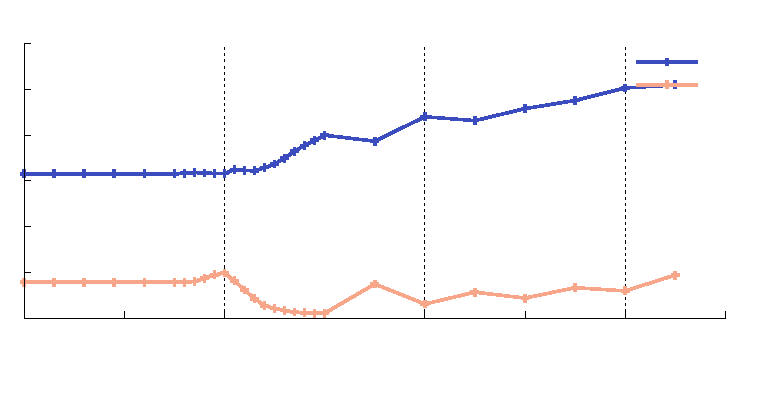
\includegraphics{99_images/201811221433-05-se-con-post-totals-lpz_c_E}}%
    \gplfronttext
  \end{picture}%
\endgroup
}%
  \end{figure}
\end{frame}
\begin{frame}[c]{Resultant turnover:\ outside LPZ}
  \begin{figure}[t]
    \centering
    \resizebox{0.6\textwidth}{!}{% GNUPLOT: LaTeX picture with Postscript
\begingroup
  \makeatletter
  \providecommand\color[2][]{%
    \GenericError{(gnuplot) \space\space\space\@spaces}{%
      Package color not loaded in conjunction with
      terminal option `colourtext'%
    }{See the gnuplot documentation for explanation.%
    }{Either use 'blacktext' in gnuplot or load the package
      color.sty in LaTeX.}%
    \renewcommand\color[2][]{}%
  }%
  \providecommand\includegraphics[2][]{%
    \GenericError{(gnuplot) \space\space\space\@spaces}{%
      Package graphicx or graphics not loaded%
    }{See the gnuplot documentation for explanation.%
    }{The gnuplot epslatex terminal needs graphicx.sty or graphics.sty.}%
    \renewcommand\includegraphics[2][]{}%
  }%
  \providecommand\rotatebox[2]{#2}%
  \@ifundefined{ifGPcolor}{%
    \newif\ifGPcolor
    \GPcolortrue
  }{}%
  \@ifundefined{ifGPblacktext}{%
    \newif\ifGPblacktext
    \GPblacktexttrue
  }{}%
  % define a \g@addto@macro without @ in the name:
  \let\gplgaddtomacro\g@addto@macro
  % define empty templates for all commands taking text:
  \gdef\gplbacktext{}%
  \gdef\gplfronttext{}%
  \makeatother
  \ifGPblacktext
    % no textcolor at all
    \def\colorrgb#1{}%
    \def\colorgray#1{}%
  \else
    % gray or color?
    \ifGPcolor
      \def\colorrgb#1{\color[rgb]{#1}}%
      \def\colorgray#1{\color[gray]{#1}}%
      \expandafter\def\csname LTw\endcsname{\color{white}}%
      \expandafter\def\csname LTb\endcsname{\color{black}}%
      \expandafter\def\csname LTa\endcsname{\color{black}}%
      \expandafter\def\csname LT0\endcsname{\color[rgb]{1,0,0}}%
      \expandafter\def\csname LT1\endcsname{\color[rgb]{0,1,0}}%
      \expandafter\def\csname LT2\endcsname{\color[rgb]{0,0,1}}%
      \expandafter\def\csname LT3\endcsname{\color[rgb]{1,0,1}}%
      \expandafter\def\csname LT4\endcsname{\color[rgb]{0,1,1}}%
      \expandafter\def\csname LT5\endcsname{\color[rgb]{1,1,0}}%
      \expandafter\def\csname LT6\endcsname{\color[rgb]{0,0,0}}%
      \expandafter\def\csname LT7\endcsname{\color[rgb]{1,0.3,0}}%
      \expandafter\def\csname LT8\endcsname{\color[rgb]{0.5,0.5,0.5}}%
    \else
      % gray
      \def\colorrgb#1{\color{black}}%
      \def\colorgray#1{\color[gray]{#1}}%
      \expandafter\def\csname LTw\endcsname{\color{white}}%
      \expandafter\def\csname LTb\endcsname{\color{black}}%
      \expandafter\def\csname LTa\endcsname{\color{black}}%
      \expandafter\def\csname LT0\endcsname{\color{black}}%
      \expandafter\def\csname LT1\endcsname{\color{black}}%
      \expandafter\def\csname LT2\endcsname{\color{black}}%
      \expandafter\def\csname LT3\endcsname{\color{black}}%
      \expandafter\def\csname LT4\endcsname{\color{black}}%
      \expandafter\def\csname LT5\endcsname{\color{black}}%
      \expandafter\def\csname LT6\endcsname{\color{black}}%
      \expandafter\def\csname LT7\endcsname{\color{black}}%
      \expandafter\def\csname LT8\endcsname{\color{black}}%
    \fi
  \fi
    \setlength{\unitlength}{0.0500bp}%
    \ifx\gptboxheight\undefined%
      \newlength{\gptboxheight}%
      \newlength{\gptboxwidth}%
      \newsavebox{\gptboxtext}%
    \fi%
    \setlength{\fboxrule}{0.5pt}%
    \setlength{\fboxsep}{1pt}%
\begin{picture}(7936.00,2550.00)%
    \gplgaddtomacro\gplbacktext{%
    }%
    \gplgaddtomacro\gplfronttext{%
    }%
    \gplgaddtomacro\gplbacktext{%
    }%
    \gplgaddtomacro\gplfronttext{%
    }%
    \gplgaddtomacro\gplbacktext{%
    }%
    \gplgaddtomacro\gplfronttext{%
    }%
    \gplbacktext
    \put(0,0){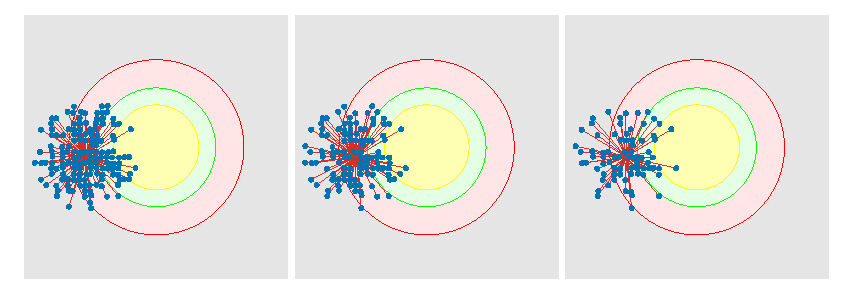
\includegraphics{99_images/201811221433-75-conns-top-EE-p_lpz_E-in}}%
    \gplfronttext
  \end{picture}%
\endgroup
}\\%
    \resizebox{0.6\textwidth}{!}{% GNUPLOT: LaTeX picture with Postscript
\begingroup
  \makeatletter
  \providecommand\color[2][]{%
    \GenericError{(gnuplot) \space\space\space\@spaces}{%
      Package color not loaded in conjunction with
      terminal option `colourtext'%
    }{See the gnuplot documentation for explanation.%
    }{Either use 'blacktext' in gnuplot or load the package
      color.sty in LaTeX.}%
    \renewcommand\color[2][]{}%
  }%
  \providecommand\includegraphics[2][]{%
    \GenericError{(gnuplot) \space\space\space\@spaces}{%
      Package graphicx or graphics not loaded%
    }{See the gnuplot documentation for explanation.%
    }{The gnuplot epslatex terminal needs graphicx.sty or graphics.sty.}%
    \renewcommand\includegraphics[2][]{}%
  }%
  \providecommand\rotatebox[2]{#2}%
  \@ifundefined{ifGPcolor}{%
    \newif\ifGPcolor
    \GPcolortrue
  }{}%
  \@ifundefined{ifGPblacktext}{%
    \newif\ifGPblacktext
    \GPblacktexttrue
  }{}%
  % define a \g@addto@macro without @ in the name:
  \let\gplgaddtomacro\g@addto@macro
  % define empty templates for all commands taking text:
  \gdef\gplbacktext{}%
  \gdef\gplfronttext{}%
  \makeatother
  \ifGPblacktext
    % no textcolor at all
    \def\colorrgb#1{}%
    \def\colorgray#1{}%
  \else
    % gray or color?
    \ifGPcolor
      \def\colorrgb#1{\color[rgb]{#1}}%
      \def\colorgray#1{\color[gray]{#1}}%
      \expandafter\def\csname LTw\endcsname{\color{white}}%
      \expandafter\def\csname LTb\endcsname{\color{black}}%
      \expandafter\def\csname LTa\endcsname{\color{black}}%
      \expandafter\def\csname LT0\endcsname{\color[rgb]{1,0,0}}%
      \expandafter\def\csname LT1\endcsname{\color[rgb]{0,1,0}}%
      \expandafter\def\csname LT2\endcsname{\color[rgb]{0,0,1}}%
      \expandafter\def\csname LT3\endcsname{\color[rgb]{1,0,1}}%
      \expandafter\def\csname LT4\endcsname{\color[rgb]{0,1,1}}%
      \expandafter\def\csname LT5\endcsname{\color[rgb]{1,1,0}}%
      \expandafter\def\csname LT6\endcsname{\color[rgb]{0,0,0}}%
      \expandafter\def\csname LT7\endcsname{\color[rgb]{1,0.3,0}}%
      \expandafter\def\csname LT8\endcsname{\color[rgb]{0.5,0.5,0.5}}%
    \else
      % gray
      \def\colorrgb#1{\color{black}}%
      \def\colorgray#1{\color[gray]{#1}}%
      \expandafter\def\csname LTw\endcsname{\color{white}}%
      \expandafter\def\csname LTb\endcsname{\color{black}}%
      \expandafter\def\csname LTa\endcsname{\color{black}}%
      \expandafter\def\csname LT0\endcsname{\color{black}}%
      \expandafter\def\csname LT1\endcsname{\color{black}}%
      \expandafter\def\csname LT2\endcsname{\color{black}}%
      \expandafter\def\csname LT3\endcsname{\color{black}}%
      \expandafter\def\csname LT4\endcsname{\color{black}}%
      \expandafter\def\csname LT5\endcsname{\color{black}}%
      \expandafter\def\csname LT6\endcsname{\color{black}}%
      \expandafter\def\csname LT7\endcsname{\color{black}}%
      \expandafter\def\csname LT8\endcsname{\color{black}}%
    \fi
  \fi
    \setlength{\unitlength}{0.0500bp}%
    \ifx\gptboxheight\undefined%
      \newlength{\gptboxheight}%
      \newlength{\gptboxwidth}%
      \newsavebox{\gptboxtext}%
    \fi%
    \setlength{\fboxrule}{0.5pt}%
    \setlength{\fboxsep}{1pt}%
\begin{picture}(7936.00,2550.00)%
    \gplgaddtomacro\gplbacktext{%
    }%
    \gplgaddtomacro\gplfronttext{%
    }%
    \gplgaddtomacro\gplbacktext{%
    }%
    \gplgaddtomacro\gplfronttext{%
    }%
    \gplgaddtomacro\gplbacktext{%
    }%
    \gplgaddtomacro\gplfronttext{%
    }%
    \gplbacktext
    \put(0,0){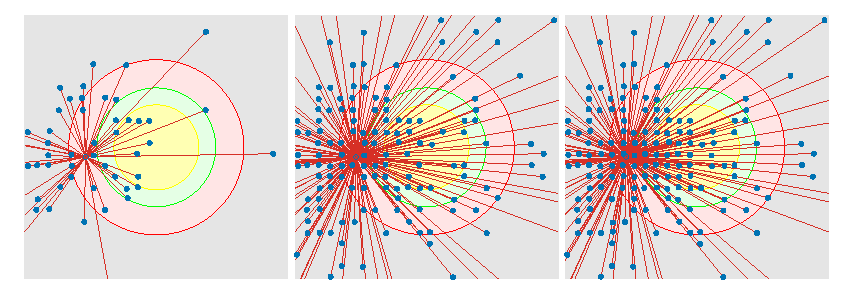
\includegraphics{99_images/201811221433-75-conns-top-IE-p_lpz_E-in}}%
    \gplfronttext
  \end{picture}%
\endgroup
}\\%
    \resizebox{0.6\textwidth}{!}{% GNUPLOT: LaTeX picture with Postscript
\begingroup
  \makeatletter
  \providecommand\color[2][]{%
    \GenericError{(gnuplot) \space\space\space\@spaces}{%
      Package color not loaded in conjunction with
      terminal option `colourtext'%
    }{See the gnuplot documentation for explanation.%
    }{Either use 'blacktext' in gnuplot or load the package
      color.sty in LaTeX.}%
    \renewcommand\color[2][]{}%
  }%
  \providecommand\includegraphics[2][]{%
    \GenericError{(gnuplot) \space\space\space\@spaces}{%
      Package graphicx or graphics not loaded%
    }{See the gnuplot documentation for explanation.%
    }{The gnuplot epslatex terminal needs graphicx.sty or graphics.sty.}%
    \renewcommand\includegraphics[2][]{}%
  }%
  \providecommand\rotatebox[2]{#2}%
  \@ifundefined{ifGPcolor}{%
    \newif\ifGPcolor
    \GPcolortrue
  }{}%
  \@ifundefined{ifGPblacktext}{%
    \newif\ifGPblacktext
    \GPblacktexttrue
  }{}%
  % define a \g@addto@macro without @ in the name:
  \let\gplgaddtomacro\g@addto@macro
  % define empty templates for all commands taking text:
  \gdef\gplbacktext{}%
  \gdef\gplfronttext{}%
  \makeatother
  \ifGPblacktext
    % no textcolor at all
    \def\colorrgb#1{}%
    \def\colorgray#1{}%
  \else
    % gray or color?
    \ifGPcolor
      \def\colorrgb#1{\color[rgb]{#1}}%
      \def\colorgray#1{\color[gray]{#1}}%
      \expandafter\def\csname LTw\endcsname{\color{white}}%
      \expandafter\def\csname LTb\endcsname{\color{black}}%
      \expandafter\def\csname LTa\endcsname{\color{black}}%
      \expandafter\def\csname LT0\endcsname{\color[rgb]{1,0,0}}%
      \expandafter\def\csname LT1\endcsname{\color[rgb]{0,1,0}}%
      \expandafter\def\csname LT2\endcsname{\color[rgb]{0,0,1}}%
      \expandafter\def\csname LT3\endcsname{\color[rgb]{1,0,1}}%
      \expandafter\def\csname LT4\endcsname{\color[rgb]{0,1,1}}%
      \expandafter\def\csname LT5\endcsname{\color[rgb]{1,1,0}}%
      \expandafter\def\csname LT6\endcsname{\color[rgb]{0,0,0}}%
      \expandafter\def\csname LT7\endcsname{\color[rgb]{1,0.3,0}}%
      \expandafter\def\csname LT8\endcsname{\color[rgb]{0.5,0.5,0.5}}%
    \else
      % gray
      \def\colorrgb#1{\color{black}}%
      \def\colorgray#1{\color[gray]{#1}}%
      \expandafter\def\csname LTw\endcsname{\color{white}}%
      \expandafter\def\csname LTb\endcsname{\color{black}}%
      \expandafter\def\csname LTa\endcsname{\color{black}}%
      \expandafter\def\csname LT0\endcsname{\color{black}}%
      \expandafter\def\csname LT1\endcsname{\color{black}}%
      \expandafter\def\csname LT2\endcsname{\color{black}}%
      \expandafter\def\csname LT3\endcsname{\color{black}}%
      \expandafter\def\csname LT4\endcsname{\color{black}}%
      \expandafter\def\csname LT5\endcsname{\color{black}}%
      \expandafter\def\csname LT6\endcsname{\color{black}}%
      \expandafter\def\csname LT7\endcsname{\color{black}}%
      \expandafter\def\csname LT8\endcsname{\color{black}}%
    \fi
  \fi
    \setlength{\unitlength}{0.0500bp}%
    \ifx\gptboxheight\undefined%
      \newlength{\gptboxheight}%
      \newlength{\gptboxwidth}%
      \newsavebox{\gptboxtext}%
    \fi%
    \setlength{\fboxrule}{0.5pt}%
    \setlength{\fboxsep}{1pt}%
\begin{picture}(7200.00,3600.00)%
    \gplgaddtomacro\gplbacktext{%
      \csname LTb\endcsname%
      \put(-60,704){\makebox(0,0)[r]{\strut{}$0$}}%
      \put(-60,996){\makebox(0,0)[r]{\strut{}$20000$}}%
      \put(-60,1289){\makebox(0,0)[r]{\strut{}$40000$}}%
      \put(-60,1581){\makebox(0,0)[r]{\strut{}$60000$}}%
      \put(-60,1873){\makebox(0,0)[r]{\strut{}$80000$}}%
      \put(-60,2166){\makebox(0,0)[r]{\strut{}$100000$}}%
      \put(-60,2458){\makebox(0,0)[r]{\strut{}$120000$}}%
      \put(-60,2750){\makebox(0,0)[r]{\strut{}$140000$}}%
      \put(-60,3043){\makebox(0,0)[r]{\strut{}$160000$}}%
      \put(-60,3335){\makebox(0,0)[r]{\strut{}$180000$}}%
      \put(72,484){\makebox(0,0){\strut{}$0$}}%
      \put(1034,484){\makebox(0,0){\strut{}$1000$}}%
      \put(1995,484){\makebox(0,0){\strut{}$2000$}}%
      \put(2957,484){\makebox(0,0){\strut{}$3000$}}%
      \put(3918,484){\makebox(0,0){\strut{}$4000$}}%
      \put(4880,484){\makebox(0,0){\strut{}$5000$}}%
      \put(5841,484){\makebox(0,0){\strut{}$6000$}}%
      \put(6803,484){\makebox(0,0){\strut{}$7000$}}%
    }%
    \gplgaddtomacro\gplfronttext{%
      \csname LTb\endcsname%
      \put(-1094,2019){\rotatebox{-270}{\makebox(0,0){\strut{}Total Synaptic elements}}}%
      \put(3437,154){\makebox(0,0){\strut{}Time (\(s\))}}%
      \put(3437,3225){\makebox(0,0){\strut{}}}%
      \csname LTb\endcsname%
      \put(5816,3162){\makebox(0,0)[r]{\strut{}Exc}}%
      \csname LTb\endcsname%
      \put(5816,2942){\makebox(0,0)[r]{\strut{}Inh}}%
    }%
    \gplbacktext
    \put(0,0){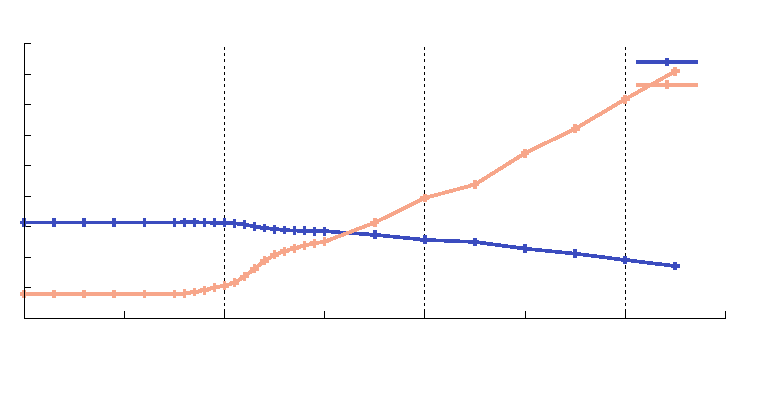
\includegraphics{99_images/201811221433-05-se-con-post-totals-p_lpz_E}}%
    \gplfronttext
  \end{picture}%
\endgroup
}
  \end{figure}
\end{frame}
\begin{frame}[c]{Pre-synaptic growth dynamics}
  \begin{columns}
    \begin{column}{0.5\textwidth}
      \begin{figure}[h]
        \begin{tikzpicture}[scale=1, transform shape]
  \begin{axis}[
    no markers, domain=-0:20, samples=100,
    y label style={rotate=-90},
    x axis line style={->},
    y axis line style={<->},
    ymin=-2.0, ymax=3.0,
    axis x line*=center,
    axis y line*=left,
    xlabel={\([Ca^{2+}]\)}, ylabel={\(\frac{dz}{dt}\)},
    grid=major, ytick={0}, xtick=\empty, clip=false,
    axis on top,
    height=6cm, width=\textwidth, enlargelimits=false
    ]
    \addplot [thick, red] {gaussnew(1,2.0, 10.0, 0.001)};
    \addplot [thick, blue] {gaussnew(1,10.0, 18.0, 0.001)};

    \draw [thick, dashed, -] (axis cs:10.0, -2.0)--(axis cs:10.0, 2.1);
    \node [above] at (axis cs:10.0, 2.2){\(\psi\)};
    \node [above, red] at (axis cs:7.5, 2.1){\(z_I\)};
    \node [above, blue] at (axis cs:12.5, 2.1){\(z_E\)};

  \end{axis}
\end{tikzpicture}


      \end{figure}
    \end{column}
    \begin{column}{0.6\textwidth}
      \centering
      \begin{itemize}
        \item Extra activity: sprouting of E
        \item Less activity: sprouting of I
      \end{itemize}
    \end{column}
  \end{columns}
\end{frame}
\begin{frame}[c]{Resultant turnover:\ pre-synaptic}
  \begin{figure}[!t]
    \centering
    \resizebox{0.6\textwidth}{!}{% GNUPLOT: LaTeX picture with Postscript
\begingroup
  \makeatletter
  \providecommand\color[2][]{%
    \GenericError{(gnuplot) \space\space\space\@spaces}{%
      Package color not loaded in conjunction with
      terminal option `colourtext'%
    }{See the gnuplot documentation for explanation.%
    }{Either use 'blacktext' in gnuplot or load the package
      color.sty in LaTeX.}%
    \renewcommand\color[2][]{}%
  }%
  \providecommand\includegraphics[2][]{%
    \GenericError{(gnuplot) \space\space\space\@spaces}{%
      Package graphicx or graphics not loaded%
    }{See the gnuplot documentation for explanation.%
    }{The gnuplot epslatex terminal needs graphicx.sty or graphics.sty.}%
    \renewcommand\includegraphics[2][]{}%
  }%
  \providecommand\rotatebox[2]{#2}%
  \@ifundefined{ifGPcolor}{%
    \newif\ifGPcolor
    \GPcolortrue
  }{}%
  \@ifundefined{ifGPblacktext}{%
    \newif\ifGPblacktext
    \GPblacktexttrue
  }{}%
  % define a \g@addto@macro without @ in the name:
  \let\gplgaddtomacro\g@addto@macro
  % define empty templates for all commands taking text:
  \gdef\gplbacktext{}%
  \gdef\gplfronttext{}%
  \makeatother
  \ifGPblacktext
    % no textcolor at all
    \def\colorrgb#1{}%
    \def\colorgray#1{}%
  \else
    % gray or color?
    \ifGPcolor
      \def\colorrgb#1{\color[rgb]{#1}}%
      \def\colorgray#1{\color[gray]{#1}}%
      \expandafter\def\csname LTw\endcsname{\color{white}}%
      \expandafter\def\csname LTb\endcsname{\color{black}}%
      \expandafter\def\csname LTa\endcsname{\color{black}}%
      \expandafter\def\csname LT0\endcsname{\color[rgb]{1,0,0}}%
      \expandafter\def\csname LT1\endcsname{\color[rgb]{0,1,0}}%
      \expandafter\def\csname LT2\endcsname{\color[rgb]{0,0,1}}%
      \expandafter\def\csname LT3\endcsname{\color[rgb]{1,0,1}}%
      \expandafter\def\csname LT4\endcsname{\color[rgb]{0,1,1}}%
      \expandafter\def\csname LT5\endcsname{\color[rgb]{1,1,0}}%
      \expandafter\def\csname LT6\endcsname{\color[rgb]{0,0,0}}%
      \expandafter\def\csname LT7\endcsname{\color[rgb]{1,0.3,0}}%
      \expandafter\def\csname LT8\endcsname{\color[rgb]{0.5,0.5,0.5}}%
    \else
      % gray
      \def\colorrgb#1{\color{black}}%
      \def\colorgray#1{\color[gray]{#1}}%
      \expandafter\def\csname LTw\endcsname{\color{white}}%
      \expandafter\def\csname LTb\endcsname{\color{black}}%
      \expandafter\def\csname LTa\endcsname{\color{black}}%
      \expandafter\def\csname LT0\endcsname{\color{black}}%
      \expandafter\def\csname LT1\endcsname{\color{black}}%
      \expandafter\def\csname LT2\endcsname{\color{black}}%
      \expandafter\def\csname LT3\endcsname{\color{black}}%
      \expandafter\def\csname LT4\endcsname{\color{black}}%
      \expandafter\def\csname LT5\endcsname{\color{black}}%
      \expandafter\def\csname LT6\endcsname{\color{black}}%
      \expandafter\def\csname LT7\endcsname{\color{black}}%
      \expandafter\def\csname LT8\endcsname{\color{black}}%
    \fi
  \fi
    \setlength{\unitlength}{0.0500bp}%
    \ifx\gptboxheight\undefined%
      \newlength{\gptboxheight}%
      \newlength{\gptboxwidth}%
      \newsavebox{\gptboxtext}%
    \fi%
    \setlength{\fboxrule}{0.5pt}%
    \setlength{\fboxsep}{1pt}%
\begin{picture}(7936.00,2550.00)%
    \gplgaddtomacro\gplbacktext{%
    }%
    \gplgaddtomacro\gplfronttext{%
    }%
    \gplgaddtomacro\gplbacktext{%
    }%
    \gplgaddtomacro\gplfronttext{%
    }%
    \gplgaddtomacro\gplbacktext{%
    }%
    \gplgaddtomacro\gplfronttext{%
    }%
    \gplbacktext
    \put(0,0){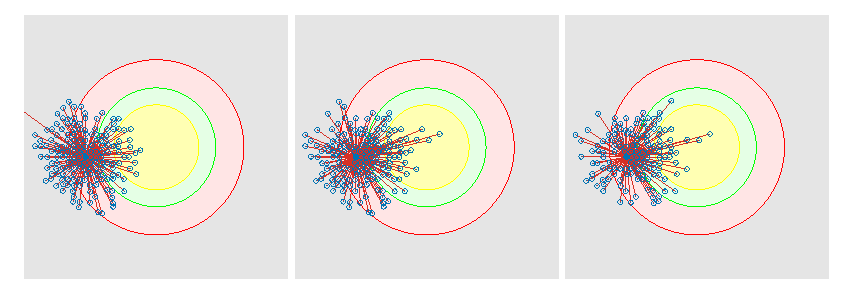
\includegraphics{99_images/201811221433-75-conns-top-EE-p_lpz_E-out}}%
    \gplfronttext
  \end{picture}%
\endgroup
}\\%
    \resizebox{0.6\textwidth}{!}{% GNUPLOT: LaTeX picture with Postscript
\begingroup
  \makeatletter
  \providecommand\color[2][]{%
    \GenericError{(gnuplot) \space\space\space\@spaces}{%
      Package color not loaded in conjunction with
      terminal option `colourtext'%
    }{See the gnuplot documentation for explanation.%
    }{Either use 'blacktext' in gnuplot or load the package
      color.sty in LaTeX.}%
    \renewcommand\color[2][]{}%
  }%
  \providecommand\includegraphics[2][]{%
    \GenericError{(gnuplot) \space\space\space\@spaces}{%
      Package graphicx or graphics not loaded%
    }{See the gnuplot documentation for explanation.%
    }{The gnuplot epslatex terminal needs graphicx.sty or graphics.sty.}%
    \renewcommand\includegraphics[2][]{}%
  }%
  \providecommand\rotatebox[2]{#2}%
  \@ifundefined{ifGPcolor}{%
    \newif\ifGPcolor
    \GPcolortrue
  }{}%
  \@ifundefined{ifGPblacktext}{%
    \newif\ifGPblacktext
    \GPblacktexttrue
  }{}%
  % define a \g@addto@macro without @ in the name:
  \let\gplgaddtomacro\g@addto@macro
  % define empty templates for all commands taking text:
  \gdef\gplbacktext{}%
  \gdef\gplfronttext{}%
  \makeatother
  \ifGPblacktext
    % no textcolor at all
    \def\colorrgb#1{}%
    \def\colorgray#1{}%
  \else
    % gray or color?
    \ifGPcolor
      \def\colorrgb#1{\color[rgb]{#1}}%
      \def\colorgray#1{\color[gray]{#1}}%
      \expandafter\def\csname LTw\endcsname{\color{white}}%
      \expandafter\def\csname LTb\endcsname{\color{black}}%
      \expandafter\def\csname LTa\endcsname{\color{black}}%
      \expandafter\def\csname LT0\endcsname{\color[rgb]{1,0,0}}%
      \expandafter\def\csname LT1\endcsname{\color[rgb]{0,1,0}}%
      \expandafter\def\csname LT2\endcsname{\color[rgb]{0,0,1}}%
      \expandafter\def\csname LT3\endcsname{\color[rgb]{1,0,1}}%
      \expandafter\def\csname LT4\endcsname{\color[rgb]{0,1,1}}%
      \expandafter\def\csname LT5\endcsname{\color[rgb]{1,1,0}}%
      \expandafter\def\csname LT6\endcsname{\color[rgb]{0,0,0}}%
      \expandafter\def\csname LT7\endcsname{\color[rgb]{1,0.3,0}}%
      \expandafter\def\csname LT8\endcsname{\color[rgb]{0.5,0.5,0.5}}%
    \else
      % gray
      \def\colorrgb#1{\color{black}}%
      \def\colorgray#1{\color[gray]{#1}}%
      \expandafter\def\csname LTw\endcsname{\color{white}}%
      \expandafter\def\csname LTb\endcsname{\color{black}}%
      \expandafter\def\csname LTa\endcsname{\color{black}}%
      \expandafter\def\csname LT0\endcsname{\color{black}}%
      \expandafter\def\csname LT1\endcsname{\color{black}}%
      \expandafter\def\csname LT2\endcsname{\color{black}}%
      \expandafter\def\csname LT3\endcsname{\color{black}}%
      \expandafter\def\csname LT4\endcsname{\color{black}}%
      \expandafter\def\csname LT5\endcsname{\color{black}}%
      \expandafter\def\csname LT6\endcsname{\color{black}}%
      \expandafter\def\csname LT7\endcsname{\color{black}}%
      \expandafter\def\csname LT8\endcsname{\color{black}}%
    \fi
  \fi
    \setlength{\unitlength}{0.0500bp}%
    \ifx\gptboxheight\undefined%
      \newlength{\gptboxheight}%
      \newlength{\gptboxwidth}%
      \newsavebox{\gptboxtext}%
    \fi%
    \setlength{\fboxrule}{0.5pt}%
    \setlength{\fboxsep}{1pt}%
\begin{picture}(7936.00,2550.00)%
    \gplgaddtomacro\gplbacktext{%
    }%
    \gplgaddtomacro\gplfronttext{%
    }%
    \gplgaddtomacro\gplbacktext{%
    }%
    \gplgaddtomacro\gplfronttext{%
    }%
    \gplgaddtomacro\gplbacktext{%
    }%
    \gplgaddtomacro\gplfronttext{%
    }%
    \gplbacktext
    \put(0,0){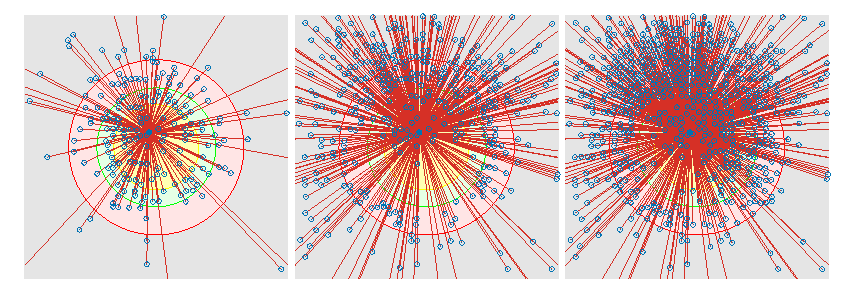
\includegraphics{99_images/201811221433-75-conns-top-IE-lpz_c_I-out}}%
    \gplfronttext
  \end{picture}%
\endgroup
}\\%
    \resizebox{0.6\textwidth}{!}{% GNUPLOT: LaTeX picture with Postscript
\begingroup
  \makeatletter
  \providecommand\color[2][]{%
    \GenericError{(gnuplot) \space\space\space\@spaces}{%
      Package color not loaded in conjunction with
      terminal option `colourtext'%
    }{See the gnuplot documentation for explanation.%
    }{Either use 'blacktext' in gnuplot or load the package
      color.sty in LaTeX.}%
    \renewcommand\color[2][]{}%
  }%
  \providecommand\includegraphics[2][]{%
    \GenericError{(gnuplot) \space\space\space\@spaces}{%
      Package graphicx or graphics not loaded%
    }{See the gnuplot documentation for explanation.%
    }{The gnuplot epslatex terminal needs graphicx.sty or graphics.sty.}%
    \renewcommand\includegraphics[2][]{}%
  }%
  \providecommand\rotatebox[2]{#2}%
  \@ifundefined{ifGPcolor}{%
    \newif\ifGPcolor
    \GPcolortrue
  }{}%
  \@ifundefined{ifGPblacktext}{%
    \newif\ifGPblacktext
    \GPblacktexttrue
  }{}%
  % define a \g@addto@macro without @ in the name:
  \let\gplgaddtomacro\g@addto@macro
  % define empty templates for all commands taking text:
  \gdef\gplbacktext{}%
  \gdef\gplfronttext{}%
  \makeatother
  \ifGPblacktext
    % no textcolor at all
    \def\colorrgb#1{}%
    \def\colorgray#1{}%
  \else
    % gray or color?
    \ifGPcolor
      \def\colorrgb#1{\color[rgb]{#1}}%
      \def\colorgray#1{\color[gray]{#1}}%
      \expandafter\def\csname LTw\endcsname{\color{white}}%
      \expandafter\def\csname LTb\endcsname{\color{black}}%
      \expandafter\def\csname LTa\endcsname{\color{black}}%
      \expandafter\def\csname LT0\endcsname{\color[rgb]{1,0,0}}%
      \expandafter\def\csname LT1\endcsname{\color[rgb]{0,1,0}}%
      \expandafter\def\csname LT2\endcsname{\color[rgb]{0,0,1}}%
      \expandafter\def\csname LT3\endcsname{\color[rgb]{1,0,1}}%
      \expandafter\def\csname LT4\endcsname{\color[rgb]{0,1,1}}%
      \expandafter\def\csname LT5\endcsname{\color[rgb]{1,1,0}}%
      \expandafter\def\csname LT6\endcsname{\color[rgb]{0,0,0}}%
      \expandafter\def\csname LT7\endcsname{\color[rgb]{1,0.3,0}}%
      \expandafter\def\csname LT8\endcsname{\color[rgb]{0.5,0.5,0.5}}%
    \else
      % gray
      \def\colorrgb#1{\color{black}}%
      \def\colorgray#1{\color[gray]{#1}}%
      \expandafter\def\csname LTw\endcsname{\color{white}}%
      \expandafter\def\csname LTb\endcsname{\color{black}}%
      \expandafter\def\csname LTa\endcsname{\color{black}}%
      \expandafter\def\csname LT0\endcsname{\color{black}}%
      \expandafter\def\csname LT1\endcsname{\color{black}}%
      \expandafter\def\csname LT2\endcsname{\color{black}}%
      \expandafter\def\csname LT3\endcsname{\color{black}}%
      \expandafter\def\csname LT4\endcsname{\color{black}}%
      \expandafter\def\csname LT5\endcsname{\color{black}}%
      \expandafter\def\csname LT6\endcsname{\color{black}}%
      \expandafter\def\csname LT7\endcsname{\color{black}}%
      \expandafter\def\csname LT8\endcsname{\color{black}}%
    \fi
  \fi
    \setlength{\unitlength}{0.0500bp}%
    \ifx\gptboxheight\undefined%
      \newlength{\gptboxheight}%
      \newlength{\gptboxwidth}%
      \newsavebox{\gptboxtext}%
    \fi%
    \setlength{\fboxrule}{0.5pt}%
    \setlength{\fboxsep}{1pt}%
\begin{picture}(7200.00,3600.00)%
    \gplgaddtomacro\gplbacktext{%
      \csname LTb\endcsname%
      \put(-60,704){\makebox(0,0)[r]{\strut{}$0$}}%
      \put(-60,967){\makebox(0,0)[r]{\strut{}$10000$}}%
      \put(-60,1230){\makebox(0,0)[r]{\strut{}$20000$}}%
      \put(-60,1493){\makebox(0,0)[r]{\strut{}$30000$}}%
      \put(-60,1756){\makebox(0,0)[r]{\strut{}$40000$}}%
      \put(-60,2020){\makebox(0,0)[r]{\strut{}$50000$}}%
      \put(-60,2283){\makebox(0,0)[r]{\strut{}$60000$}}%
      \put(-60,2546){\makebox(0,0)[r]{\strut{}$70000$}}%
      \put(-60,2809){\makebox(0,0)[r]{\strut{}$80000$}}%
      \put(-60,3072){\makebox(0,0)[r]{\strut{}$90000$}}%
      \put(-60,3335){\makebox(0,0)[r]{\strut{}$100000$}}%
      \put(72,484){\makebox(0,0){\strut{}$0$}}%
      \put(1034,484){\makebox(0,0){\strut{}$1000$}}%
      \put(1995,484){\makebox(0,0){\strut{}$2000$}}%
      \put(2957,484){\makebox(0,0){\strut{}$3000$}}%
      \put(3918,484){\makebox(0,0){\strut{}$4000$}}%
      \put(4880,484){\makebox(0,0){\strut{}$5000$}}%
      \put(5841,484){\makebox(0,0){\strut{}$6000$}}%
      \put(6803,484){\makebox(0,0){\strut{}$7000$}}%
    }%
    \gplgaddtomacro\gplfronttext{%
      \csname LTb\endcsname%
      \put(-1094,2019){\rotatebox{-270}{\makebox(0,0){\strut{}Total Synaptic elements}}}%
      \put(3437,154){\makebox(0,0){\strut{}Time (\(s\))}}%
      \put(3437,3225){\makebox(0,0){\strut{}}}%
      \csname LTb\endcsname%
      \put(5816,3162){\makebox(0,0)[r]{\strut{}Exc}}%
      \csname LTb\endcsname%
      \put(5816,2942){\makebox(0,0)[r]{\strut{}Inh}}%
    }%
    \gplbacktext
    \put(0,0){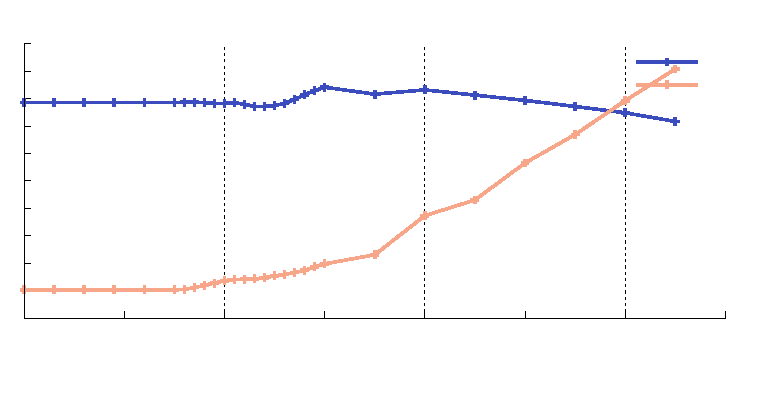
\includegraphics{99_images/201811221433-05-se-con-pre-totals-lpz_c_I-p_lpz_E}}%
    \gplfronttext
  \end{picture}%
\endgroup
}
  \end{figure}
\end{frame}
\begin{frame}[c]{Post-synaptic growth dynamics}
  \begin{columns}
    \begin{column}{0.5\textwidth}
      \begin{figure}[h]
        \begin{tikzpicture}[scale=1, transform shape]
  \begin{axis}[
    no markers, domain=-0:20, samples=100,
    y label style={rotate=-90},
    x axis line style={->},
    y axis line style={<->},
    ymin=-2.0, ymax=3.0,
    axis x line*=center,
    axis y line*=left,
    xlabel={\([Ca^{2+}]\)}, ylabel={\(\frac{dz}{dt}\)},
    grid=major, ytick={0}, xtick=\empty, clip=false,
    axis on top,
    height=6.0cm, width=\textwidth, enlargelimits=false
    ]
    \addplot [thick, blue] {gaussnew(1,5.0, 10.0,1)};
    \addplot [thick, red] {gaussnew(1,10.0, 15.0,1)};

    \draw [thick, dashed, -] (axis cs:10.0, -2.0)--(axis cs:10.0, 2.1);
    \node [above] at (axis cs:10.0, 2.2){\(\psi\)};
    \node [above, blue] at (axis cs:7.5, 2.1){\(z_E\)};
    \node [above, red] at (axis cs:12.5, 2.1){\(z_I\)};

  \end{axis}
\end{tikzpicture}

      \end{figure}
    \end{column}
    \begin{column}{0.6\textwidth}
      \centering
      \begin{itemize}
        \item Loss of activity: sprouting of E, retraction of I
        \item Extra activity: retraction of E, sprouting of I
      \end{itemize}
    \end{column}
  \end{columns}
\end{frame}
\begin{frame}[c]{Post-synaptic dynamics: single neuron stability}
  \begin{columns}
    \begin{column}{0.5\textwidth}
      \begin{figure}[h]
        \centering
        \resizebox{\textwidth}{!}{% http://www.texample.net/tikz/examples/degree-wheel/
\def\radiuslines{2.5cm}
\def\radiuscircle{0.4cm}
\def\onedegrad{1.8cm}
\def\fivedegrad{1.75cm}
\def\tendegrad{1.7cm}
\def\circlex{2.0}
\def\circley{4}

\begin{tikzpicture}[scale=1.2, transform shape]
  \draw (\circlex, \circley) circle (\radiuscircle);

  \foreach \angle in {120, 122.5,...,180} \draw [blue] ([shift=(\angle:\radiuscircle + 0.1cm )] \circlex, \circley) -- ++ (\angle:\radiuscircle+\radiuslines);
  \foreach \angle in {190,200,...,240} \draw [red] ([shift=(\angle:\radiuscircle + 0.1cm)] \circlex, \circley) -- ++ (\angle:\radiuscircle+\radiuslines);

  \node[left, blue] at (1,7.5) {\(Den_{ex}\)};
  \node[left, red] at (1,0.5) {\(Den_{in}\)};

  \draw [-{Latex[length=2mm]}] (\circlex,1.4) -- ++ (0, 2.0);
  \node[below] at (\circlex,1.0) {\(I_{ext}\)};
  % sine wave inside a circle node
  % https://tex.stackexchange.com/a/257613/11281
  \node[below, draw,circle,inner sep=-0.4pt] at (\circlex, 1.2)
  {\tikz \draw[scale=0.05,domain=-3.141:3.141,smooth,variable=\t]
  plot (\t,{sin(\t r)});};

  \draw [-{Latex[length=2mm]}] (2.5, \circley) -- ++ (1.2 , 0);
  \node[right] at (3.7, \circley) {\([Ca^{2+}]\)};


\end{tikzpicture}
}%
      \end{figure}
    \end{column}
    \begin{column}{0.5\textwidth}
      \begin{figure}[h]
        \centering
        \resizebox{0.9\textwidth}{!}{% GNUPLOT: LaTeX picture with Postscript
\begingroup
  \makeatletter
  \providecommand\color[2][]{%
    \GenericError{(gnuplot) \space\space\space\@spaces}{%
      Package color not loaded in conjunction with
      terminal option `colourtext'%
    }{See the gnuplot documentation for explanation.%
    }{Either use 'blacktext' in gnuplot or load the package
      color.sty in LaTeX.}%
    \renewcommand\color[2][]{}%
  }%
  \providecommand\includegraphics[2][]{%
    \GenericError{(gnuplot) \space\space\space\@spaces}{%
      Package graphicx or graphics not loaded%
    }{See the gnuplot documentation for explanation.%
    }{The gnuplot epslatex terminal needs graphicx.sty or graphics.sty.}%
    \renewcommand\includegraphics[2][]{}%
  }%
  \providecommand\rotatebox[2]{#2}%
  \@ifundefined{ifGPcolor}{%
    \newif\ifGPcolor
    \GPcolortrue
  }{}%
  \@ifundefined{ifGPblacktext}{%
    \newif\ifGPblacktext
    \GPblacktexttrue
  }{}%
  % define a \g@addto@macro without @ in the name:
  \let\gplgaddtomacro\g@addto@macro
  % define empty templates for all commands taking text:
  \gdef\gplbacktext{}%
  \gdef\gplfronttext{}%
  \makeatother
  \ifGPblacktext
    % no textcolor at all
    \def\colorrgb#1{}%
    \def\colorgray#1{}%
  \else
    % gray or color?
    \ifGPcolor
      \def\colorrgb#1{\color[rgb]{#1}}%
      \def\colorgray#1{\color[gray]{#1}}%
      \expandafter\def\csname LTw\endcsname{\color{white}}%
      \expandafter\def\csname LTb\endcsname{\color{black}}%
      \expandafter\def\csname LTa\endcsname{\color{black}}%
      \expandafter\def\csname LT0\endcsname{\color[rgb]{1,0,0}}%
      \expandafter\def\csname LT1\endcsname{\color[rgb]{0,1,0}}%
      \expandafter\def\csname LT2\endcsname{\color[rgb]{0,0,1}}%
      \expandafter\def\csname LT3\endcsname{\color[rgb]{1,0,1}}%
      \expandafter\def\csname LT4\endcsname{\color[rgb]{0,1,1}}%
      \expandafter\def\csname LT5\endcsname{\color[rgb]{1,1,0}}%
      \expandafter\def\csname LT6\endcsname{\color[rgb]{0,0,0}}%
      \expandafter\def\csname LT7\endcsname{\color[rgb]{1,0.3,0}}%
      \expandafter\def\csname LT8\endcsname{\color[rgb]{0.5,0.5,0.5}}%
    \else
      % gray
      \def\colorrgb#1{\color{black}}%
      \def\colorgray#1{\color[gray]{#1}}%
      \expandafter\def\csname LTw\endcsname{\color{white}}%
      \expandafter\def\csname LTb\endcsname{\color{black}}%
      \expandafter\def\csname LTa\endcsname{\color{black}}%
      \expandafter\def\csname LT0\endcsname{\color{black}}%
      \expandafter\def\csname LT1\endcsname{\color{black}}%
      \expandafter\def\csname LT2\endcsname{\color{black}}%
      \expandafter\def\csname LT3\endcsname{\color{black}}%
      \expandafter\def\csname LT4\endcsname{\color{black}}%
      \expandafter\def\csname LT5\endcsname{\color{black}}%
      \expandafter\def\csname LT6\endcsname{\color{black}}%
      \expandafter\def\csname LT7\endcsname{\color{black}}%
      \expandafter\def\csname LT8\endcsname{\color{black}}%
    \fi
  \fi
    \setlength{\unitlength}{0.0500bp}%
    \ifx\gptboxheight\undefined%
      \newlength{\gptboxheight}%
      \newlength{\gptboxwidth}%
      \newsavebox{\gptboxtext}%
    \fi%
    \setlength{\fboxrule}{0.5pt}%
    \setlength{\fboxsep}{1pt}%
\begin{picture}(3400.00,2550.00)%
    \gplgaddtomacro\gplbacktext{%
      \csname LTb\endcsname%
      \put(-98,704){\makebox(0,0)[r]{\strut{}$18$}}%
      \put(-98,1178){\makebox(0,0)[r]{\strut{}$21$}}%
      \put(-98,1653){\makebox(0,0)[r]{\strut{}$24$}}%
      \put(-98,2127){\makebox(0,0)[r]{\strut{}$27$}}%
      \put(34,484){\makebox(0,0){\strut{}$0$}}%
      \put(962,484){\makebox(0,0){\strut{}$250$}}%
      \put(1890,484){\makebox(0,0){\strut{}$500$}}%
      \put(2817,484){\makebox(0,0){\strut{}$750$}}%
    }%
    \gplgaddtomacro\gplfronttext{%
      \csname LTb\endcsname%
      \put(-604,1494){\rotatebox{-270}{\makebox(0,0){\strut{}\([Ca^{2+}]\)}}}%
      \put(1518,154){\makebox(0,0){\strut{}Time (\(s\))}}%
      \put(1518,2175){\makebox(0,0){\strut{}}}%
    }%
    \gplbacktext
    \put(0,0){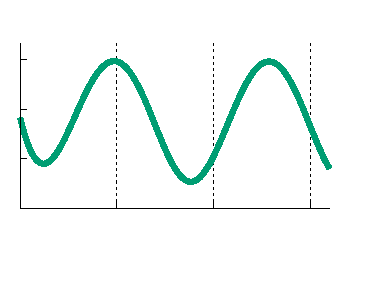
\includegraphics{99_images/single-neuron-calciums}}%
    \gplfronttext
  \end{picture}%
\endgroup
}\\%
        \resizebox{0.9\textwidth}{!}{% GNUPLOT: LaTeX picture with Postscript
\begingroup
  \makeatletter
  \providecommand\color[2][]{%
    \GenericError{(gnuplot) \space\space\space\@spaces}{%
      Package color not loaded in conjunction with
      terminal option `colourtext'%
    }{See the gnuplot documentation for explanation.%
    }{Either use 'blacktext' in gnuplot or load the package
      color.sty in LaTeX.}%
    \renewcommand\color[2][]{}%
  }%
  \providecommand\includegraphics[2][]{%
    \GenericError{(gnuplot) \space\space\space\@spaces}{%
      Package graphicx or graphics not loaded%
    }{See the gnuplot documentation for explanation.%
    }{The gnuplot epslatex terminal needs graphicx.sty or graphics.sty.}%
    \renewcommand\includegraphics[2][]{}%
  }%
  \providecommand\rotatebox[2]{#2}%
  \@ifundefined{ifGPcolor}{%
    \newif\ifGPcolor
    \GPcolortrue
  }{}%
  \@ifundefined{ifGPblacktext}{%
    \newif\ifGPblacktext
    \GPblacktexttrue
  }{}%
  % define a \g@addto@macro without @ in the name:
  \let\gplgaddtomacro\g@addto@macro
  % define empty templates for all commands taking text:
  \gdef\gplbacktext{}%
  \gdef\gplfronttext{}%
  \makeatother
  \ifGPblacktext
    % no textcolor at all
    \def\colorrgb#1{}%
    \def\colorgray#1{}%
  \else
    % gray or color?
    \ifGPcolor
      \def\colorrgb#1{\color[rgb]{#1}}%
      \def\colorgray#1{\color[gray]{#1}}%
      \expandafter\def\csname LTw\endcsname{\color{white}}%
      \expandafter\def\csname LTb\endcsname{\color{black}}%
      \expandafter\def\csname LTa\endcsname{\color{black}}%
      \expandafter\def\csname LT0\endcsname{\color[rgb]{1,0,0}}%
      \expandafter\def\csname LT1\endcsname{\color[rgb]{0,1,0}}%
      \expandafter\def\csname LT2\endcsname{\color[rgb]{0,0,1}}%
      \expandafter\def\csname LT3\endcsname{\color[rgb]{1,0,1}}%
      \expandafter\def\csname LT4\endcsname{\color[rgb]{0,1,1}}%
      \expandafter\def\csname LT5\endcsname{\color[rgb]{1,1,0}}%
      \expandafter\def\csname LT6\endcsname{\color[rgb]{0,0,0}}%
      \expandafter\def\csname LT7\endcsname{\color[rgb]{1,0.3,0}}%
      \expandafter\def\csname LT8\endcsname{\color[rgb]{0.5,0.5,0.5}}%
    \else
      % gray
      \def\colorrgb#1{\color{black}}%
      \def\colorgray#1{\color[gray]{#1}}%
      \expandafter\def\csname LTw\endcsname{\color{white}}%
      \expandafter\def\csname LTb\endcsname{\color{black}}%
      \expandafter\def\csname LTa\endcsname{\color{black}}%
      \expandafter\def\csname LT0\endcsname{\color{black}}%
      \expandafter\def\csname LT1\endcsname{\color{black}}%
      \expandafter\def\csname LT2\endcsname{\color{black}}%
      \expandafter\def\csname LT3\endcsname{\color{black}}%
      \expandafter\def\csname LT4\endcsname{\color{black}}%
      \expandafter\def\csname LT5\endcsname{\color{black}}%
      \expandafter\def\csname LT6\endcsname{\color{black}}%
      \expandafter\def\csname LT7\endcsname{\color{black}}%
      \expandafter\def\csname LT8\endcsname{\color{black}}%
    \fi
  \fi
    \setlength{\unitlength}{0.0500bp}%
    \ifx\gptboxheight\undefined%
      \newlength{\gptboxheight}%
      \newlength{\gptboxwidth}%
      \newsavebox{\gptboxtext}%
    \fi%
    \setlength{\fboxrule}{0.5pt}%
    \setlength{\fboxsep}{1pt}%
\begin{picture}(3400.00,2550.00)%
    \gplgaddtomacro\gplbacktext{%
      \csname LTb\endcsname%
      \put(-98,704){\makebox(0,0)[r]{\strut{}-$200$}}%
      \put(-98,1080){\makebox(0,0)[r]{\strut{}-$100$}}%
      \put(-98,1457){\makebox(0,0)[r]{\strut{}$0$}}%
      \put(-98,1833){\makebox(0,0)[r]{\strut{}$100$}}%
      \put(-98,2210){\makebox(0,0)[r]{\strut{}$200$}}%
      \put(34,484){\makebox(0,0){\strut{}$0$}}%
      \put(962,484){\makebox(0,0){\strut{}$250$}}%
      \put(1890,484){\makebox(0,0){\strut{}$500$}}%
      \put(2817,484){\makebox(0,0){\strut{}$750$}}%
    }%
    \gplgaddtomacro\gplfronttext{%
      \csname LTb\endcsname%
      \put(-668,1494){\rotatebox{-270}{\makebox(0,0){\strut{}\(\Delta~g (nS)\)}}}%
      \put(1518,154){\makebox(0,0){\strut{}Time (\(s\))}}%
      \put(1518,2175){\makebox(0,0){\strut{}}}%
      \csname LTb\endcsname%
      \put(306,2112){\makebox(0,0)[r]{\strut{}E}}%
      \csname LTb\endcsname%
      \put(1293,2112){\makebox(0,0)[r]{\strut{}I}}%
      \csname LTb\endcsname%
      \put(2280,2112){\makebox(0,0)[r]{\strut{}Net}}%
    }%
    \gplbacktext
    \put(0,0){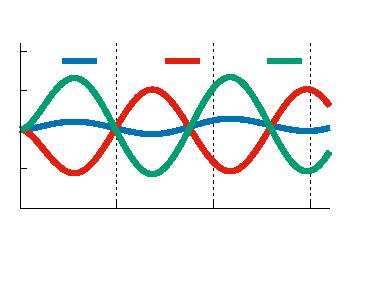
\includegraphics{99_images/single-neuron-inputs-new}}%
    \gplfronttext
  \end{picture}%
\endgroup
}\\%
      \end{figure}
    \end{column}
  \end{columns}
\end{frame}
\begin{frame}[c]{Conclusions}
  \begin{itemize}
    \item New model: biologically realistic.
    \item Replicates experimental observations:
      \begin{itemize}
        \item Ingrowth of excitatory axons to LPZ\@.
        \item Outgrowth of inhibitory axons from LPZ\@.
          \pause{}
        \item Massive disinhibition in LPZ\@.
        \item Role of inhibition in structural plasticity as a controller of critical time window?
      \end{itemize}
      \pause{}
    \item Suggests:
      \begin{itemize}
        \item Activity dependent dynamics for synaptic structures.
        \item Single neuron stabilisation by structural plasticity.
      \end{itemize}
  \end{itemize}
\end{frame}
\begin{frame}[c]{Now what?}
  \begin{itemize}
    \item Functional implications of structural plasticity? Associative memory?
      \pause{}
    \item Application of growth dynamics to multi-compartmental neuron models?
      \pause{}
    \item Faithful modelling of cytoskeleton modification (actin)?
  \end{itemize}
\end{frame}
\end{document}
